%%%%%%%% ICLR 2026 SUBMISSION FILE %%%%%%%%%%%%%%%%%

\documentclass{article}

\PassOptionsToPackage{dvipsnames}{xcolor}

% Anonymous review mode is the default; final-copy mode remains disabled.
\usepackage{iclr2026_conference,times}

% Recommended packages:
\usepackage[utf8]{inputenc}
\usepackage[T1]{fontenc}
\IfFileExists{microtype.sty}{\usepackage{microtype}}{}
\usepackage{graphicx}
\usepackage{tikz}
\usetikzlibrary{arrows.meta,calc,positioning}
\usepackage{subcaption}
\usepackage{booktabs}
\usepackage{tabularx}
\usepackage{xcolor}
\usepackage{hyperref}
\hypersetup{
  pdftitle={Finite-Reference Error Bounds for Recurrent Evaluators in Policy Improvement},
  pdfauthor={},
  pdfcreator={},
  pdfproducer={},
  hidelinks
}

\providecommand{\theHalgorithm}{\arabic{algorithm}}

% Math and theorems
\usepackage{amsmath}
\usepackage{amssymb}
\usepackage{mathtools}
\usepackage{amsthm}

% Algorithms
\usepackage{algorithm}
\usepackage{algorithmic}

% For itemize options
\usepackage{enumitem}

% Mild line-breaking allowance only.
\emergencystretch=1em


%%%%%%%%%%%%%%%%%%%%%%%%%%%%
% THEOREMS
%%%%%%%%%%%%%%%%%%%%%%%%%%%%
\theoremstyle{plain}
\newtheorem{theorem}{Theorem}[section]
\newtheorem{proposition}[theorem]{Proposition}
\newtheorem{lemma}[theorem]{Lemma}
\newtheorem{corollary}[theorem]{Corollary}
\theoremstyle{definition}
\newtheorem{definition}[theorem]{Definition}
\newtheorem{assumption}[theorem]{Assumption}
\theoremstyle{remark}
\newtheorem{remark}[theorem]{Remark}

\newtheorem*{theorem*}{Theorem}
\newtheorem*{proposition*}{Proposition}
\newtheorem*{lemma*}{Lemma}
\newtheorem{example}[theorem]{Example}


\newcommand{\missingfigurebox}[1]{%
  \fbox{\parbox{0.78\linewidth}{\centering\footnotesize #1}}%
}

%%%%%%%%%%%%%%%%%%%%%%%%%%%%
% CUSTOM MACROS
%%%%%%%%%%%%%%%%%%%%%%%%%%%%
\newcommand{\R}{\mathbb{R}}
\newcommand{\E}{\mathbb{E}}
\newcommand{\XX}{\mathcal{X}}
\newcommand{\YY}{\mathcal{Y}}
\newcommand{\ZZ}{\mathcal{Z}}
\newcommand{\SSS}{\mathcal{S}}
\newcommand{\AAcal}{\mathcal{A}}
\newcommand{\norm}[1]{\left\lVert #1 \right\rVert}
\newcommand{\Lip}{\mathrm{Lip}}
\newcommand{\KL}{\mathrm{KL}}
\newcommand{\sg}{\operatorname{sg}}
\newcommand{\Cdrift}{C_{\mathrm{drift}}}
% NEW: Notation for policy-specific sup-norms
\newcommand{\supnorm}[2]{\left\| #1 \right\|_{\infty,#2}}

% ========================================
% Collaborative comments (OFF by default for anonymous submission)
% ========================================
\newif\ifcomments
\commentsfalse % SUBMISSION: keep OFF (set \commentstrue only for internal drafts)
\ifcomments
  \PackageWarningNoLine{main}{COMMENTS ARE ENABLED. Set commentsfalse before submission.}
  \newcommand{\revA}[1]{{\color{red}\small[A: #1]}}
  \newcommand{\revB}[1]{{\color{blue}\small[B: #1]}}
  \newcommand{\revC}[1]{{\color{green}\small[C: #1]}}
  \newcommand{\revD}[1]{{\color{Mulberry}\small[D: #1]}}
\else
  \newcommand{\revA}[1]{}
  \newcommand{\revB}[1]{}
  \newcommand{\revC}[1]{}
  \newcommand{\revD}[1]{}
\fi

%%%%%%%%%%%%%%%%%%%%%%%%%%%%
% TITLE & AUTHOR
%%%%%%%%%%%%%%%%%%%%%%%%%%%%

\title{Finite-Reference Error Bounds for Recurrent Evaluators in Policy Improvement}

\author{%
  Anonymous Author(s)
}

\begin{document}

\maketitle
\begin{abstract}
We study fixed-snapshot error bounds for a finite-depth recurrent value evaluator inside policy improvement. For finite reference depths $m>n$, value error is controlled by the depth discrepancy $\|U_n-U_m\|$ and a Bellman residual at depth $m$; a recurrent path bounds the first term without assuming a latent fixed point. For an edit budget $H$, a stagewise analysis replaces the infinite-horizon residual factor by $(1-\gamma^{K\lceil h/K\rceil})/(1-\gamma^K)$ at clock $h$. Persistent latents use the clock-complete augmented state $(x,y,z,h)$ and one shared frozen recurrent transition map. We also give finite-horizon conservative-policy-improvement bounds under exact statewise centering and exact probability-space mixing, plus a deployment perturbation bound under a uniform total-variation or KL condition. Finite-state regression tests check the theorem pipeline and boundary cases; they are not learned-model validation. The retained $4\times4$ Sudoku records are in-sample, unmatched, or missing reconstructible checkpoints, so we make no historical performance comparison. Finite-batch diagnostics do not instantiate the uniform theorem assumptions.
\end{abstract}

\section{Introduction}
\label{sec:intro}

Tiny Recursive Models (TRMs)~\citep{TRM2025} obtain predictions through iterative latent refinement. In checker-guided tasks such as Sudoku, the same recurrent computation can serve as an internal evaluator for candidate edits to a partial plan. A finite unroll can be useful while remaining transient: there is no general reason for an arbitrary TRM to be designed around convergence to a latent fixed point. Standard approximate-policy-iteration and conservative-policy-improvement (CPI) analyses~\citep{BertsekasTsitsiklis1996,KakadeLangford2002} place evaluator error in a black-box term and therefore do not distinguish a finite recurrent path from a Bellman residual at a chosen reference depth.

We analyze Unrolled Policy Iteration with TRMs (UPI--TRM), which retains the inner recurrence, uses a scalar value head to score candidate plan edits, and places environment transitions only in the outer checker-guided MDP. The analysis fixes the MDP, recurrence, value head, initialization, and policy pair. It is not an end-to-end theorem for SGD, TD learning, BPTT, or distillation. Euclidean projection can supply forward invariance, and exact baseline summation can supply the statewise centering needed by the CPI step, but these are conditions on a frozen snapshot rather than guarantees about how training reaches it.

Our primary result (Theorem~\ref{thm:finite_reference_depth}) compares $U_n(s)=V_\psi(z^{(n)}(s),x)$ with any deeper finite reference $U_m$, bounding $\|U_n-V^\pi\|$ by $\|U_n-U_m\|$ plus the Bellman residual of $U_m$. No recurrent convergence is assumed. The finite-horizon specialization in Theorem~\ref{thm:finite_horizon_reference} uses the edit clock and exact absorbing boundary to replace the infinite geometric tail by the number of remaining $K$-step blocks. Theorem~\ref{thm:finite_horizon_cpi} gives time-indexed CPI constants, and Theorem~\ref{thm:deployment_perturbation} quantifies the gap between the exact mixture and a separately deployed policy. These are conditional fixed-snapshot results, not training guarantees.

The evidence has two distinct roles. First, an exactly solvable finite MDP numerically unit-tests the composed value, advantage, and CPI inequalities; it is not an empirical discovery. Second, retained hard-$4\times4$ Sudoku artifacts document historical implementations. The episodic aggregate records $0\%$ success over 10 seeds, but the retained endpoint rows do not identify the evaluated policy. Historical persistent logs and configuration metadata record training-population reuse and parameter interpolation rather than the exact pointwise mixture. The checkpoints, hard-suite dataset, ordered evaluation population, exact training revision, and exact environment-interaction counters are absent. We therefore exclude the old performance and ablation tables and attach no comparative or inferential interpretation to those records.

\textbf{Scope.} Write $h$ for the remaining edit budget. Episodic latents are Markov on $s=(x,y,h)$. At a fixed snapshot, persistent latents are Markov on the clock-complete state $\bar s=(x,y,z,h)$. Their direct residual certificate needs no latent fixed point or slow drift; slow drift is needed only for the stronger comparison with a memoryless fixed-point reference. Repository audit found that the historical persistent path omitted the carried latent from replay updates, omitted the edit clock from recorded state, and used parameter interpolation for deployment. The hard-suite data and checkpoints are absent, so the original runs cannot be re-executed. The current empirical domain is only $4\times4$ Sudoku.

\textbf{Contributions.}
\begin{itemize}[leftmargin=1.2em,topsep=0pt,itemsep=2pt]
\item Fixed-point-free finite-reference value and path bounds, including a finite-horizon sharpening with exact terminal handling (Theorems~\ref{thm:finite_reference_depth} and~\ref{thm:finite_horizon_reference}).
\item A direct finite-depth certificate for persistent state on the augmented MDP, separated from an optional slow-drift comparison (Corollary~\ref{cor:persistent_cpi_augmented}).
\item Finite-horizon CPI under exact centering and exact mixing, with TV/KL perturbation bounds for a deployed policy (Theorems~\ref{thm:finite_horizon_cpi} and~\ref{thm:deployment_perturbation}).
\item Deterministic theorem-pipeline regression tests and an evidence audit that excludes unsupported historical performance claims.
\end{itemize}

\begin{figure}[t]
\centering
\resizebox{0.82\linewidth}{!}{\begin{tikzpicture}[
  >=Stealth,
  font=\small,
  panel/.style={draw, rounded corners=3pt, line width=0.5pt, inner sep=6pt, align=left},
  leftpanel/.style={panel, fill=orange!10, text width=4.5cm},
  rightpanel/.style={panel, fill=blue!8, text width=4.9cm},
  flow/.style={->, thick, black},
  map/.style={->, thick, black},
  note/.style={font=\scriptsize, align=center, text width=2.0cm, text=black}
]

\node[font=\bfseries\small] at (-2.8, 2.85) {Original TRM};
\node[font=\bfseries\small] at (4.6, 2.85) {Clock-complete edit MDP};
\draw[dashed, gray!60] (0.9, -3.0) -- (0.9, 3.1);

\node[leftpanel] (inner) at (-2.8, 1.25) {%
\textbf{Inner refinement}\\[-1pt]
Refine latent state from input $x$ and plan $y_t$.\\[2pt]
{\centering $z^{(k+1)} = f_\theta(z^{(k)}, y_t, x)$\par}
};

\node[leftpanel] (outer) at (-2.8, -1.85) {%
\textbf{Outer refinement}\\[-1pt]
Iterate the inner refinement across multiple passes of $f_\theta$, continuously refining the current answer $y_t$.
};

\draw[flow] (inner.south) -- node[right, note] {latent\\drives $y_t$} (outer.north);

\node[rightpanel] (eval) at (4.6, 1.25) {%
\textbf{Internal evaluator}\\[-1pt]
Unroll the evaluator for depth $n$.\\[2pt]
{\centering
$\begin{aligned}
z^{(k+1)} &= (\Pi_R \circ f_\theta)(z^{(k)}, y_t, x)\\
U_n(s_t) &= V_\psi(z_t^{(n)},x,y_t)\\
\widetilde U_n(\bar s_t) &= V_\psi(z_t^{(n)},x,y_t)
\end{aligned}$\par
}
};

\node[rightpanel] (mdp) at (4.6, -1.85) {%
\textbf{Clock-complete state}\\[-1pt]
Episodic: $s_t=(x,y_t,h_t)$\\
Persistent: $\bar s_t=(x,y_t,z_t,h_t)$\\
Edit: $y_{t+1}=\mathrm{edit}(y_t,a_t;x)$\\
Clock: $h_{t+1}=h_t-1$
};

\draw[flow] (eval.south) -- node[right, note] {policy uses\\finite-depth value} (mdp.north);

\draw[map] (inner.east) -- node[above, note] {inner loop\\$\mapsto$ evaluator depth} (eval.west);
\draw[map] (outer.east) -- node[below, note] {outer refinement\\$\mapsto$ edit MDP} (mdp.west);

\end{tikzpicture}
}
\caption{TRM-to-MDP bridge used throughout the paper. Left: the original TRM's inner latent-refinement loop nested inside its outer continuous refinement of the current answer $y_t$~\citep{TRM2025}. Right: we swap TRM's continuous outer refinement for a discrete plan-edit loop under checker feedback and treat the inner loop as an internal evaluator unrolled for depth $n$. The episodic Markov state is $(x,y_t,h_t)$; carrying the latent requires the augmented state $(x,y_t,z_t,h_t)$. The checker maps to reward, and $h_t$ records the remaining edit budget.}
\label{fig:trm_architecture}
\end{figure}

\section{Related Work}
\label{sec:related_work}

\textbf{Recursive latent reasoning models.}
TRMs~\citep{TRM2025} and Hierarchical Reasoning Models~\citep{HRM2025} use iterative latent refinement for structured reasoning; follow-up work studies training dynamics and test-time adaptation~\citep{Qasim2025CGAR,McGovern2025TRMAdapt}. We keep TRM's inner latent refinement but swap its supervised outer loop for a discrete plan-edit loop under checker feedback, and analyze how finite inner evaluation affects policy improvement. The contraction assumption is DEQ-adjacent~\citep{Bai2019DEQ} only in providing a regime with bounded truncation bias.

\textbf{Policy-improvement analyses.}
CPI, TRPO, and safe/monotone policy improvement~\citep{KakadeLangford2002,Schulman2015TRPO,Pirotta2013SafePI,Metelli2021SafePI,Eshwar2025MonotoneCPI} all bound improvement under an abstract evaluation-error term, but treat that error as a single black-box quantity. The closest formal neighbor is function-approximation CPI~\citep{Metelli2021SafePI,Eshwar2025MonotoneCPI}, which relates a learned $V_\psi$ to $V^\pi$ via a regression model, a sampling distribution, and an optimizer. We do something orthogonal: conditional on sup-norm residual and centering control, we expose the finite recurrent path between depths $n$ and $m$. A contractive recurrence turns this path into an $L_z^n$ specialization, but contraction is not required by the primary result. Empirical RLVR work on LLM reasoning~\citep{Wang2025OneShotRLVR,Su2025RewardBridge,DeepSeekR1} uses verifiable rewards in a similar spirit but does not analyze approximation error. A quantitative join with FA-CPI on $V_\psi$ would need coverage and uniform-convergence assumptions we leave out.

\textbf{Planning and structured-decision neighbors.}
Sequence-model RL ranges from architecture-level planning~\citep{Tamar2016VIN} and inference-time search~\citep{janner2021trajectory} to pure sequence modeling~\citep{chen2021decision,laskin2022context}; structured prediction and Sudoku/constraint RL~\citep{Daume2009SEARN,Ross2011DAgger,Chang2015LOLS,Mehta2021SudokuRL,Klein2022SudokuRL} are closer to our plan-space MDP framing. The TRM inner unroll differs from both: it is architecture-internal computation within one state evaluation.

\section{Background and Setup}
\label{sec:setup}


The original TRM, given input $x$ and plan $y_t$, runs an inner loop that updates a latent $z^{(k+1)} = f_\theta(z^{(k)}, y_t, x)$. After $n$ steps it reads out a refined prediction from a task head trained on checker-labeled puzzles~\citep{TRM2025}. UPI--TRM keeps $f_\theta$ but replaces the task head with two pieces. The first is an optional projection $\Pi_R$ that keeps latents inside a radius-$R$ ball (Assumption~\ref{ass:Lip}, Eq.~\ref{eq:projection}), so the projected update is
\(
z^{(k+1)} = (\Pi_R \circ f_\theta)(z^{(k)}, y_t, x).
\)
The second is a scalar value head $V_\psi$ that produces the unrolled evaluator output $U_n(s_t)=V_\psi(z_t^{(n)},x)$ with episodic state $s_t=(x,y_t,h_t)$, where $h_t$ is the remaining edit budget, and scores candidate plans in the outer CPI loop.

In the plan-space MDP the external episodic state is $s_t=(x,y_t,h_t)$, the action is an edit $a_t$, and a nonterminal transition sets $y_{t+1}=\mathrm{edit}(y_t,a_t;x)$ and $h_{t+1}=h_t-1$; solving, a terminal STOP action, or exhausting the budget sends the process to $s_{\mathrm{abs}}$. Budget exhaustion is treated as termination, not as a separately bootstrapped truncation. A checker score $c(x,y)$ supplies reward, optionally via potential shaping~\citep{Ng1999Shaping} $r=r_0+\gamma\Phi(s')-\Phi(s)$ with $\Phi=c$. The latent $z$ is \emph{not} part of the environment state in the episodic analysis; it is internal computation used to evaluate $s_t$. The resulting process is a discounted MDP $(\mathcal S,\mathcal A,P,r,\rho,\gamma)$ with $\gamma\in[0,1)$ and $K\ge 1$. All theoretical statements fix one parameter snapshot: the MDP, recurrence, initialization, value head, current policy $\pi$, and candidate policy $\pi_{\mathrm{cand}}$ do not change while the displayed quantities are evaluated. The formal results assume finite or countable state and action spaces and use ordinary sup norms; the proofs also apply when only the relevant policy-pair closure and supported action sets are finite or countable. Rewards are bounded and the relevant closure is invariant under $\pi$ almost surely. This setting covers every reported experiment. Appendix~\ref{app:adv_closure_full} states the additional domination and total-variation requirements for a general-kernel extension. Increasing $n$ spends more computation inside one state evaluation but does not change the environment horizon or search depth, so the analysis tracks evaluator truncation error inside a fixed external MDP.

\textbf{Episodic-$z$ vs.\ persistent-$z$.}
In \emph{episodic-$z$}, the latent is reinitialized from the current plan at each edit step, so $s=(x,y,h)$ is Markov. In \emph{persistent-$z$}, the latent is carried across edits, matching the original TRM. With persistent latents the next-state distribution depends jointly on $(x,y,z,h)$, since the same plan paired with a different carried latent or remaining budget can produce a different policy output or termination event. Treating $(x,y)$ as the state in this regime is a non-Markov approximation. Appendix~\ref{app:persistent_latent} lifts the finite-depth residual certificate directly to $\bar s=(x,y,z,h)$; this step needs no latent fixed point or slow drift. A separate slow-drift assumption is required only for comparison with a memoryless fixed-point reference.

\textbf{Notation.}
For one common initialization $z^{(0)}(s)=z_{\mathrm{init}}(x,y)$, which deliberately ignores the clock, let $z^{(j)}(s)$ be the latent after $j$ applications of the frozen recurrent map and let $U_j(s)=V_\psi(z^{(j)}(s),x)$. At the absorbing state, every $U_j$ uses the same depth-independent normalization from Appendix~\ref{app:shaping_convention}. Only the optional contractive specialization uses the latent fixed point $z^*$ and $U_*(s)=V_\psi(z^*(s),x)$. We write $\|f\|_{\infty,\pi,\pi_{\mathrm{cand}}}^{\mathrm{adv}}:=\sup_{s\in\mathcal{R}_{\pi,\pi_{\mathrm{cand}}}^{\mathrm{adv}}\cup\{s_{\mathrm{abs}}\}}|f(s)|$ for the ordinary sup-norm over the advantage-evaluation closure used by CPI. This closure contains states reachable under $\pi$ and the one-step successors needed to evaluate actions supported by $\pi$ and $\pi_{\mathrm{cand}}$, and is invariant under subsequent $\pi$ dynamics almost surely (Appendix~\ref{app:adv_closure_full}; full notation in Appendix~\ref{app:notation}). We use one shared absorbing atom $s_{\mathrm{abs}}$ for both episodic and augmented notation.

\section{UPI--TRM Algorithm}
\label{sec:algorithm}
Algorithm~\ref{alg:upi} alternates three phases: collect edit trajectories, fit $U_n$ against a $K$-step bootstrap target, and take a conservative mixture step. The formal guarantee applies to the explicit mixture; distillation is an implementation step outside the theorem.

\begin{algorithm}[t]
\small
\caption{One UPI--TRM update on the clock-complete edit MDP}
\label{alg:upi}
\begin{algorithmic}[1]
\STATE \textbf{Initialize:} sample $x$, initialize $y_0$, set remaining budget $h_0=T$, and initialize $z_0$ for persistent-$z$
\FOR{$t=0,\dots,T-1$ until solved or $h_t=0$}
  \STATE Set $s_t=(x,y_t,h_t)$; for persistent-$z$, set $\bar s_t=(x,y_t,z_t,h_t)$
  \STATE \textbf{Latent input:} episodic-$z$ uses $z_t\gets z_{\mathrm{init}}(x,y_t)$; persistent-$z$ uses the carried pre-unroll $z_t$
  \STATE \textbf{Evaluator:} $z_t^{(n)} \gets (\Pi_R \circ f_\theta)^{\circ n}(z_t,y_t,x)$
  \STATE \textbf{Value:} $U_n(s_t)\gets V_\psi(z_t^{(n)},x)$ in episodic-$z$; $\widetilde U_n(\bar s_t)\gets V_\psi(z_t^{(n)},x)$ in persistent-$z$
  \STATE \textbf{Action:} sample $a_t\sim\pi_\phi(\cdot\mid y_t,z_t^{(n)},x)$ and apply the edit; observe $r_t$, $y_{t+1}$, and terminal flag $d_t$; set $h_{t+1}=h_t-1$
  \IF{$d_t$ or $h_{t+1}=0$}
    \STATE Store $(s_t,a_t,r_t,s_{\mathrm{abs}})$ in episodic-$z$, or $(\bar s_t,a_t,r_t,s_{\mathrm{abs}})$ in persistent-$z$
  \ELSE
    \STATE Set $s_{t+1}=(x,y_{t+1},h_{t+1})$ and $\bar s_{t+1}=(x,y_{t+1},z_t^{(n)},h_{t+1})$
    \STATE Store $(s_t,a_t,r_t,s_{t+1})$ in episodic-$z$, or $(\bar s_t,a_t,r_t,\bar s_{t+1})$ in persistent-$z$
    \STATE For persistent-$z$, carry the post-unroll latent: $z_{t+1}\gets z_t^{(n)}$
  \ENDIF
\ENDFOR
\STATE \textbf{Value update:} form $G^{(K)}$ and regress the mode-appropriate evaluator ($U_n$ or $\widetilde U_n$)
\STATE \textbf{Advantage estimate:} compute $\widehat A$ centered conditional on $s_t$, or on full $\bar s_t$ in persistent-$z$
\STATE \textbf{Policy update:} take a policy-gradient step to obtain $\pi_{\mathrm{cand}}$
\STATE \textbf{Conservative step:} $\pi_{\mathrm{new}} \gets (1-\alpha)\pi_\phi+\alpha\pi_{\mathrm{cand}}$
\STATE \textbf{Optional distillation:} distill $\pi_{\mathrm{new}}$ into a single policy network
\end{algorithmic}
\end{algorithm}

The direct episodic and augmented-state applications of Theorem~\ref{thm:monotone_with_error} require exact statewise baseline summation, the explicit mixture step, and no distillation. In the persistent case, centering and the mixture identity are conditional on the full augmented state. The explicit mixture (rather than a clipped surrogate, trust-region update, parameter interpolation, or distilled approximation) is required for the linear-in-$\alpha$ tightening; otherwise the centering defect and deployment mismatch lie outside the stated bound.

Persistent-$z$ is handled in Appendix~\ref{app:persistent_latent}, and the initialization condition in Appendix~\ref{app:implementation} gives $C_z\le 2R$. Per update, the dominant cost is $O(T \cdot |\mathcal A| \cdot n)$ inner-evaluator unrolls: $T$ states per trajectory, $|\mathcal A|$ unrolls each for exact baseline summation, and depth $n$ per unroll.



\section{Bellman Residuals and an Optional Contractive Regime}
\label{sec:contraction}
We train $U_n$ by $K$-step bootstrapped regression with loss $\mathcal{L}_{\mathrm{val}}=\E_{s_0\sim\mu}[(V_\psi(z^{(n)}(s_0),x_0)-\mathrm{sg}(G^{(K)}))^2]$, where $G^{(K)}=\sum_{k<K}\gamma^k r_k + \gamma^K \bar V(s_K)$ is the $K$-step bootstrap target. The $K$-step Bellman operator $\mathcal T^\pi_K$ is the standard $\gamma^K$-contraction with fixed point $V^\pi$~\citep{SuttonBarto2018,Puterman1994}.

The primary finite-reference-depth result in Section~\ref{sec:error_bounds} uses Bellman contraction but does not assume that the recurrent computation converges. It assumes sup-norm residual control on the relevant closure; we do not prove a general $L^2(\mu)\to\|\cdot\|_\infty$ conversion. A separate, optional assumption below makes a latent fixed-point specialization available. Bellman contraction is operator-level; inner-evaluator contraction of $z\mapsto\tilde f_\theta(z,y,x)$ controls a recurrent path within one frozen forward pass and by itself gives no TD- or training-convergence guarantee.

\begin{assumption}[Forward-invariant contraction]
\label{ass:Lip}
The latent space $\ZZ$ is a complete normed space (in our implementation, $\mathbb R^d$ with the Euclidean norm). There exists a closed set $\mathcal{Z}_{\mathrm{inv}}\subseteq\ZZ$ such that the projected update map $\tilde f_\theta(z,y,x):=(\Pi_R\circ f_\theta)(z,y,x)$ maps $\mathcal{Z}_{\mathrm{inv}}$ to itself and is an $L_z$-contraction in $z$ with $L_z\in(0,1)$.
For every $(x,y)$, the initialization satisfies $z_{\mathrm{init}}(x,y)\in\mathcal{Z}_{\mathrm{inv}}$.
Let $z^*(x,y)$ denote the unique fixed point and assume
\[
C_z:=\sup_{(x,y)}\|\tilde f_\theta(z_{\mathrm{init}}(x,y),y,x)-z_{\mathrm{init}}(x,y)\|<\infty.
\]
\end{assumption}

We enable operator-norm clamping and per-layer scaling as a contraction-oriented intervention; $\Pi_R$ provides forward invariance. The retained finite-difference quantities are local proxies and do not certify the global modulus required by Assumption~\ref{ass:Lip}. We therefore distinguish the theorem's contractive regime from the empirical \emph{clamping enabled} condition. Value-head spectral normalization is disabled in these comparisons to avoid a separate value-head confound.

The intervention is labeled \emph{clamping enabled} in empirical code and
records. That label does not imply contraction. The $L_z$-dependent theorem
terms require a certified global modulus below one, which the retained local
finite-difference measurements do not provide.

\section{Finite-Depth Evaluation Error Decomposition and CPI Penalty}
\label{sec:error_bounds}

We connect finite evaluator depth to CPI. The CPI shell is standard~\citep{KakadeLangford2002}; the TRM-specific content is a finite-reference-depth error decomposition that does not require a recurrent fixed point. We focus on episodic-$z$ and defer persistent-$z$ to Appendix~\ref{app:persistent_latent}.

\subsection{Value error bounds (episodic-$z$)}
\label{sec:value_error_bounds}

$K$-step Bellman contraction gives, for any bounded measurable $V$ on the forward-invariant closure,
\begin{equation}
\|V - V^\pi\|_{\infty,\pi,\pi_{\mathrm{cand}}}^{\mathrm{adv}}
\le
\frac{1}{1-\gamma^K}\,
\|V-\mathcal{T}^\pi_K V\|_{\infty,\pi,\pi_{\mathrm{cand}}}^{\mathrm{adv}},
\label{eq:boundA}
\end{equation}
and therefore permits any finite unroll depth to serve as the reference.

\begin{theorem}[Finite-reference-depth value decomposition]
\label{thm:finite_reference_depth}
Fix either a finite or countable MDP, or a finite or countable policy-pair closure whose action supports under $\pi$ and $\pi_{\mathrm{cand}}$ are finite or countable. Fix one frozen parameter snapshot, the policy pair $(\pi,\pi_{\mathrm{cand}})$, one measurable recurrent map shared by every depth, a common measurable initialization $z^{(0)}(s)=z_{\mathrm{init}}(x,y)$ that ignores the clock, $K\ge1$, and one latent norm on $\mathcal Z\subseteq\mathbb R^d$. Let $V_\psi:\mathcal Z\times\mathcal X\to\mathbb R$ be a measurable scalar value head. For every $j$, define $z^{(j)}$ by iterating that same map from that same initialization and set $U_j(s)=V_\psi(z^{(j)}(s),x)$. Let $\mathcal R_{\pi,\pi_{\mathrm{cand}}}^{\mathrm{adv}}\cup\{s_{\mathrm{abs}}\}$ contain the states reachable under $\pi$ and every one-step successor required by actions supported by either policy, and require it to be invariant under subsequent $\pi$ transitions almost surely. Assume rewards and $U_j$, $j\in\{n,\ldots,m\}$, are bounded on this closure; every depth uses the common boundary value $U_j(s_{\mathrm{abs}})=-C_{\max}$; and $\mathcal T_K^\pi$ maps bounded real functions on the closure to bounded real functions on the same closure. All displayed norms are ordinary sup norms on this closure. Then, for any finite integers $0\le n<m$,
\begin{align}
\|U_n - V^\pi\|_{\infty,\pi,\pi_{\mathrm{cand}}}^{\mathrm{adv}}
&\le
\underbrace{\|U_n-U_m\|_{\infty,\pi,\pi_{\mathrm{cand}}}^{\mathrm{adv}}}_{\text{finite-depth discrepancy}}
+
\underbrace{\frac{\|U_m-\mathcal T_K^\pi U_m\|_{\infty,\pi,\pi_{\mathrm{cand}}}^{\mathrm{adv}}}{1-\gamma^K}}_{\text{reference-depth residual}}.
\label{eq:finite_reference_depth}
\end{align}
If, in addition, the scalar head is $L_V$-Lipschitz in its latent argument uniformly in $x$, then
\begin{align}
\|U_n-U_m\|_{\infty,\pi,\pi_{\mathrm{cand}}}^{\mathrm{adv}}
&\le
L_V\sum_{j=n}^{m-1}
\sup_{s\in\mathcal R_{\pi,\pi_{\mathrm{cand}}}^{\mathrm{adv}}}
\|z^{(j+1)}(s)-z^{(j)}(s)\|.
\label{eq:finite_path_length}
\end{align}
\end{theorem}

The theorem is a residual bound plus a telescoping path bound; we make no novelty claim for the triangle inequality itself. Its role is to expose a certifiable finite reference $m$: the recurrence may perform useful transient computation and need not converge before, at, or after $m$. The same frozen policy $\pi$ appears in $V^\pi$ and $\mathcal T_K^\pi$, and the latter bootstraps from $U_m$ itself.

For the optional contractive specialization, additionally assume the fixed-point map is measurable and $U_*$ is bounded on the closure (the latter follows from Assumption~\ref{ass:bounded_value_head}); set $U_*(s_{\mathrm{abs}})=-C_{\max}$ and define
\begin{equation}
\varepsilon_{\mathrm{res}}^* \triangleq \|U_* - \mathcal{T}^\pi_K U_*\|_{\infty,\pi,\pi_{\mathrm{cand}}}^{\mathrm{adv}}.
\label{eq:eps_res_def}
\end{equation}
Under Assumption~\ref{ass:Lip} and the Lipschitz-head condition, consecutive latent differences satisfy
$\|z^{(j+1)}-z^{(j)}\|\le L_z^j C_z$ uniformly. Hence Theorem~\ref{thm:finite_reference_depth} gives the finite-$m$ specialization
\begin{align}
\|U_n - V^\pi\|_{\infty,\pi,\pi_{\mathrm{cand}}}^{\mathrm{adv}}
&\le
L_V C_z\frac{L_z^n(1-L_z^{m-n})}{1-L_z}
+\frac{\|U_m-\mathcal T_K^\pi U_m\|_{\infty,\pi,\pi_{\mathrm{cand}}}^{\mathrm{adv}}}{1-\gamma^K}.
\label{eq:finite_reference_contracting}
\end{align}
Uniform convergence $U_m\to U_*$ and Bellman contraction imply convergence of the residual norm. Taking $m\to\infty$ recovers
\begin{align}
\|U_n - V^\pi\|_{\infty,\pi,\pi_{\mathrm{cand}}}^{\mathrm{adv}}
\le
\underbrace{\frac{\varepsilon_{\mathrm{res}}^*}{1-\gamma^K}}_{\text{fixed-point residual}}
+
\underbrace{L_V\,\frac{L_z^{\,n}}{1-L_z}\,C_z}_{\text{geometric path bound}}.
\label{eq:epsV_dials}
\end{align}

Thus the earlier fixed-point decomposition is a specialization obtained by geometrically bounding the recurrent path and sending the finite reference depth to infinity. It is not an assertion that arbitrary TRMs are designed to converge to a fixed point. Under $\|z_{\mathrm{init}}\|_2\le R$ with $\mathcal{Z}_{\mathrm{inv}}=B_R$, projection gives $C_z\le 2R$ (Remark~\ref{rem:finite_R_Cz}).

A projection-active specialization makes the role of $R$ explicit. When all relevant pre-projection outputs satisfy $\|f_\theta(z,y,x)\|_2\ge\rho_R>R$ for $z\in B_R$, radial projection reduces the pre-projection Lipschitz upper bound by the factor $R/\rho_R$. The projected map is contractive only when $(R/\rho_R)L_z^{\mathrm{pre}}(R)<1$. Proposition~\ref{prop:proj_sat_contraction} makes this condition explicit and gives
\begin{equation}
L_z\;\le\;L_z^{\mathrm{sat}}(R)\;:=\;\frac{R}{\rho_R}\,L_z^{\mathrm{pre}}(R),
\label{eq:Lz_sat}
\end{equation}
and Proposition~\ref{prop:proj_residual_anchor} bounds the residual relative to the boundary-normalized zero-latent baseline
\[
B_0(x,y):=V_\psi(0,x),
\qquad
B_0(s_{\mathrm{abs}}):=-C_{\max}.
\]
\begin{equation}
\varepsilon_{\mathrm{res}}^*\;\le\;\varepsilon_0\;+\;(1+\gamma^K)\,L_V(R)\,R,
\label{eq:eps_res_proj}
\end{equation}
with $\varepsilon_0:=\|B_0-\mathcal{T}^\pi_K B_0\|_{\infty,\pi,\pi_{\mathrm{cand}}}^{\mathrm{adv}}$. Projection thus enters both the architectural term (through $L_V(R)R$) and the truncation term (through $L_z^{\mathrm{sat}}(R)$ and $C_z\le 2R$). The experiments report finite-sample proxies for this regime. They do not certify the uniform $\rho_R$ and Lipschitz assumptions; the finite-batch $U_n$ Bellman residual upper-bounds $\varepsilon_{\mathrm{res}}^*$ only up to the truncation gap (Remark~\ref{rem:residual_bridge}).

\begin{corollary}[Finite-depth residual certificate]
\label{cor:finite_depth_residual_certificate}
Fix a policy $\pi$ and a finite-depth evaluator $U_n$ on the advantage-evaluation closure $\mathcal{R}_{\pi,\pi_{\mathrm{cand}}}^{\mathrm{adv}}$. Define
\begin{equation}
\varepsilon_{\mathrm{res},n}
\triangleq
\|U_n-\mathcal{T}^\pi_K U_n\|_{\infty,\pi,\pi_{\mathrm{cand}}}^{\mathrm{adv}}.
\label{eq:eps_res_n_def}
\end{equation}
Then
\begin{equation}
\|U_n-V^\pi\|_{\infty,\pi,\pi_{\mathrm{cand}}}^{\mathrm{adv}}
\le
\frac{\varepsilon_{\mathrm{res},n}}{1-\gamma^K}.
\label{eq:finite_depth_residual_certificate}
\end{equation}
If $\widehat A=\widehat A_{U_n}$ is the exact one-step centered estimator of Eq.~\eqref{eq:Ahat_def_app}, then Assumption~\ref{ass:Ahat_error_bound} holds with
\begin{equation}
\varepsilon_A
\triangleq
\frac{2\gamma\,\varepsilon_{\mathrm{res},n}}{1-\gamma^K}.
\label{eq:finite_depth_residual_adv}
\end{equation}
Consequently, under the hypotheses of Theorem~\ref{thm:monotone_with_error},
\begin{equation}
\eta(\pi_{\mathrm{new}})
\ge
\widehat{L}_\pi(\pi_{\mathrm{new}})
-
\frac{2\alpha\gamma}{1-\gamma}\,
\frac{\varepsilon_{\mathrm{res},n}}{1-\gamma^K}
-
\frac{2\varepsilon_{\mathrm{CPI}}\,\gamma}{(1-\gamma)^2}\,\alpha^2.
\label{eq:finite_depth_residual_cpi}
\end{equation}
\end{corollary}

This certificate follows from Bellman contraction alone and applies in finite MDPs or deterministic edit environments where the $K$-step backup is computable. It does not require the Lipschitz or contractive architectural assumptions. A finite-MDP unit test checks 80 value/decomposition rows and 21 CPI rows with zero violations (Appendix~\ref{app:finite_mdp_certificate}).

The CPI guarantees below are deterministic conditional statements that need sup-norm residual control on $\mathcal R_{\pi,\pi_{\mathrm{cand}}}^{\mathrm{adv}}$. In finite or exactly evaluable MDPs Corollary~\ref{cor:finite_depth_residual_certificate} can certify it; otherwise it remains an assumption. Because the closure depends on both $\pi$ and $\pi_{\mathrm{cand}}$, residual control is a property of the policy pair. The certificate is post-candidate: once $\pi_{\mathrm{cand}}$ is chosen, the relevant closure can be checked; future candidates require their own check.

\begin{corollary}[Advantage-error bridge]
\label{cor:epsA_dials}
Under the hypotheses of Theorem~\ref{thm:finite_reference_depth}, define
\begin{equation}
B_{n,m}
:=
\|U_n-U_m\|_{\infty,\pi,\pi_{\mathrm{cand}}}^{\mathrm{adv}}
+
\frac{\|U_m-\mathcal T_K^\pi U_m\|_{\infty,\pi,\pi_{\mathrm{cand}}}^{\mathrm{adv}}}{1-\gamma^K}.
\label{eq:Bnm_def}
\end{equation}
Let $\widehat A=\widehat A_{U_n}$ be the exact one-step centered estimator of Eq.~\eqref{eq:Ahat_def_app}, with the transition expectation evaluated exactly (or applied to a deterministic transition) and the baseline computed exactly under $\pi$. Then Assumption~\ref{ass:Ahat_error_bound} holds with the valid choice
\begin{equation}
\varepsilon_A = 2\gamma B_{n,m}.
\label{eq:epsA_finite_reference}
\end{equation}
If Assumption~\ref{ass:Lip} and the $L_V$-Lipschitz head condition also hold, sending $m\to\infty$ gives the fixed-point specialization
\begin{align}
\varepsilon_A
&\le
\underbrace{\frac{2\gamma\,\varepsilon_{\mathrm{res}}^*}{1-\gamma^K}}_{\text{architectural}}
+
\underbrace{2\gamma\,L_V\,\frac{L_z^{\,n}}{1-L_z}\,C_z}_{\text{unrolling}}.
\label{eq:epsA_dials}
\end{align}
\end{corollary}

Here the value-error norm is taken over $\mathcal{R}^{\mathrm{adv}}_{\pi,\pi_{\mathrm{cand}}}$ (Definition~\ref{def:adv_closure}). For a centered $K$-step estimator, $2\gamma$ becomes $2\gamma^K$; GAE-style constants can likewise be absorbed into $\varepsilon_A$ (Remark~\ref{rem:A_error_kstep_app}). Combining the finite-reference choice with Theorem~\ref{thm:monotone_with_error} gives the fixed-point-free penalty
\begin{equation}
\eta(\pi_{\mathrm{new}})
\ge
\widehat L_\pi(\pi_{\mathrm{new}})
-\frac{2\alpha\gamma}{1-\gamma}B_{n,m}
-\frac{2\varepsilon_{\mathrm{CPI}}\gamma}{(1-\gamma)^2}\alpha^2.
\label{eq:finite_reference_cpi}
\end{equation}
Thus a finite recurrent path and a residual at any deeper finite depth feed directly into CPI. Geometric $L_z^n$ dependence is only the contractive specialization.


\subsection{Conservative policy improvement}
\label{sec:cpi}

For $\pi_{\mathrm{new}}=(1-\alpha)\pi+\alpha\pi_{\mathrm{cand}}$, standard CPI gives monotonic improvement up to an $O(\alpha^2)$ penalty. The decompositions above enter through centered evaluation error: under exact centering, candidate-policy advantage error contributes the explicit linear term $\alpha\,\varepsilon_{A,\mathrm{cand}}/(1-\gamma)$.
\begin{assumption}[Uniform advantage error on states visited by $\pi$]
\label{ass:Ahat_error_bound}
For some $\varepsilon_A\ge 0$:
\begin{equation}
|\widehat{A}(s,a) - A^\pi(s,a)| \le \varepsilon_A
\end{equation}
for all $(s,a)$ with $s \in \mathcal{R}_{\pi}$ and
$a \in \mathrm{supp}(\pi_{\mathrm{cand}}(\cdot|s)) \cup \mathrm{supp}(\pi(\cdot|s))$.
\end{assumption}

The relevant support depends on $\pi_{\mathrm{cand}}$ (standard CPI circularity; see Appendix~\ref{app:adv_closure_full}).
Write $\widehat{L}_\pi(\pi') := \eta(\pi) + \frac{1}{1-\gamma}\E_{s\sim d_\pi, a\sim\pi'(\cdot\mid s)}[\widehat{A}(s,a)]$ for the CPI surrogate built from the approximate advantage.

\begin{theorem}[CPI with centered evaluation error]
\label{thm:monotone_with_error}
Fix one discounted MDP with bounded rewards and a current/candidate policy pair. Let $\alpha\in[0,1]$ and let $\pi_{\mathrm{new}}=(1-\alpha)\pi+\alpha\pi_{\mathrm{cand}}$ be the exact probability-space mixture policy, with no distillation or parameter-interpolation error.
Assume the advantage estimator is statewise-centered under $\pi$:
\begin{equation}
\E_{a\sim\pi(\cdot\mid s)}[\widehat A(s,a)] = 0
\qquad\text{for all } s\in\mathcal{R}_\pi.
\label{eq:centering_condition}
\end{equation}
We define the candidate-policy bias in advantage estimation
\begin{equation}
\varepsilon_{A,\mathrm{cand}}
\triangleq
\sup_{s \in \mathcal{R}_{\pi}}
\left|
\E_{a\sim\pi_{\mathrm{cand}}(\cdot\mid s)}\!\left[\widehat{A}(s,a)-A^\pi(s,a)\right]
\right|.
\label{eq:epsA0_def}
\end{equation}
and assume $\varepsilon_{A,\mathrm{cand}}<\infty$.
Then:
\begin{equation}
\eta(\pi_{\mathrm{new}})
\ge
\widehat{L}_\pi(\pi_{\mathrm{new}})
-
\frac{\alpha}{1-\gamma}\,\varepsilon_{A,\mathrm{cand}}
-
\frac{2\varepsilon_{\mathrm{CPI}}\,\gamma}{(1-\gamma)^2}\,\alpha^2,
\label{eq:main_theorem}
\end{equation}
where $\varepsilon_{\mathrm{CPI}} \triangleq \sup_s\bigl|\E_{a\sim\pi_{\mathrm{cand}}(\cdot\mid s)}A^\pi(s,a)\bigr|$.
\end{theorem}

Assumption~\ref{ass:Ahat_error_bound} is one sufficient condition implying
$\varepsilon_{A,\mathrm{cand}}\le\varepsilon_A$; it is not otherwise required
for the central inequality~\eqref{eq:main_theorem}.

The linear-in-$\alpha$ contribution $\alpha\varepsilon_{A,\mathrm{cand}}/(1-\gamma)$, instead of the naive $\varepsilon_A/(1-\gamma)$, requires the exact-centering condition~\eqref{eq:centering_condition}. This condition holds whenever the estimator is constructed to be exactly statewise centered. For Eq.~\eqref{eq:Ahat_def_app}, the baseline expectation must be evaluated exactly; in our finite action space we use explicit summation. Sampling-based or learned approximations instead incur the centering defect of Corollary~\ref{cor:cpi_centering_defect}.

The constants split into estimable and assumed quantities
(Table~\ref{tab:diagnostics}). Local finite-difference and batch measurements
are diagnostics, not uniform bounds. In particular, the architectural residual
$\varepsilon_{\mathrm{res}}^*$ is a sup norm over the advantage closure; a
finite-batch residual relates to it only through the truncation gap in
Remark~\ref{rem:residual_bridge}. The retained historical records do not
contain the checkpoints and byte-identified diagnostic population needed to
regenerate these quantities, so calibration on the successful persistent
implementation is \emph{not verifiable from supplied evidence}.

\begin{corollary}[Sufficient condition for one-step improvement]
\label{cor:one_step_improvement_condition}
Under Theorem~\ref{thm:monotone_with_error}, if
\begin{equation}
\widehat{L}_\pi(\pi_{\mathrm{new}})-\eta(\pi)
\ge
\frac{\alpha}{1-\gamma}\,\varepsilon_{A,\mathrm{cand}}
+
\frac{2\varepsilon_{\mathrm{CPI}}\gamma}{(1-\gamma)^2}\,\alpha^2,
\label{eq:sufficient_improvement_condition}
\end{equation}
then $\eta(\pi_{\mathrm{new}})\ge \eta(\pi)$.
In particular, under Corollary~\ref{cor:epsA_dials}, it suffices to replace
$\varepsilon_{A,\mathrm{cand}}$ in~\eqref{eq:sufficient_improvement_condition}
by $2\gamma B_{n,m}$. Under the optional contractive specialization, one may further upper-bound this quantity by
\[
2\gamma\left(
\frac{\varepsilon_{\mathrm{res}}^*}{1-\gamma^K}
+
L_V\,\frac{L_z^{\,n}}{1-L_z}\,C_z
\right).
\]
\end{corollary}

Theorem~\ref{thm:monotone_with_error} applies to the exact mixture; distillation error lies outside it. Exact baseline summation over a discrete action space satisfies~\eqref{eq:centering_condition}; approximate centering replaces the linear term by $[(1-\alpha)\varepsilon_{\mathrm{cent}}+\alpha\varepsilon_{A,\mathrm{cand}}]/(1-\gamma)$ via Corollary~\ref{cor:cpi_centering_defect}. The theorem is most informative in the small-$\alpha$ regime, where the linear term dominates the $\alpha^2$ penalty.

\begin{corollary}[One-step parameter dependence]
\label{cor:cpi_dials_main}
Under Corollary~\ref{cor:epsA_dials} and Theorem~\ref{thm:monotone_with_error},
\begin{align}
\eta(\pi_{\mathrm{new}})
&\ge
\widehat{L}_\pi(\pi_{\mathrm{new}})
-
\frac{2\alpha\gamma}{1-\gamma}
\left(
\frac{\varepsilon_{\mathrm{res}}^*}{1-\gamma^K}
+
L_V\,\frac{L_z^{\,n}}{1-L_z}\,C_z
\right)
-
\frac{2\varepsilon_{\mathrm{CPI}}\,\gamma}{(1-\gamma)^2}\,\alpha^2.
\label{eq:main_bound_dials}
\end{align}
\end{corollary}

Corollary~\ref{cor:cpi_dials_main} is the optional fixed-point specialization of the finite-reference penalty $2\alpha\gamma B_{n,m}/(1-\gamma)$. It makes the one-step dependence on $(L_z,n,K,\alpha)$ explicit. For $n\ge1$, its recurrent term vanishes as $L_z\to0$; together with $\varepsilon_{\mathrm{res}}^*\to0$, this recovers the standard CPI expression. At $n=0$, the displayed recurrent term instead tends to $L_VC_z$ and no such claim is made. The retained finite-difference values are local proxies and certify no global modulus below one. On the hard suite, we therefore treat the $L_z$-dependent terms as monitoring quantities.

A projection-aware version of \eqref{eq:main_bound_dials} substitutes $\varepsilon_0+(1+\gamma^K)L_V(R)R$ for $\varepsilon_{\mathrm{res}}^*$ and $L_z^{\mathrm{sat}}(R)$ for $L_z$; the full statement is Eq.~\eqref{eq:main_bound_proj} in Appendix~\ref{app:projection_theory}. The saturated-regime upper bound depends multiplicatively on both $R/\rho_R$ and $L_z^{\mathrm{pre}}(R)$, and the retained local proxies certify neither global factor. For $n\ge1$, a smaller certified $L_z$ or larger $n$ reduces $L_z^n$; smaller $\alpha$ is safer; larger $K$ tightens $1/(1-\gamma^K)$ at the cost of a $K$-dependent residual. Persistent-$z$ uses the direct augmented-state residual of Appendix~\ref{app:persistent_latent}; slow drift enters only the optional comparison to a memoryless fixed-point reference.

\section{Evidence Status and Numerical Unit Test}
\label{sec:experiments}

All learned-model task records concern $4\times4$ Sudoku. None provides a
held-out, interaction-matched method comparison or empirical validation of the
fixed-snapshot theorem. Table~\ref{tab:claim_status} maps each retained claim
to its required conditions and evidence status.

\paragraph{Historical limitations.}
The successful persistent record used parameter interpolation, evaluated
training records, omitted the carried latent from replay updates, and omitted
the remaining-edit clock from the recorded state. The historical persistent
checkpoints, hard-suite data, ordered outcomes, and producer revision are
absent. Its held-out performance interpretation and theorem-facing diagnostics
are therefore \emph{not verifiable from supplied evidence}. Historical projection/clamping
and baseline aggregates are excluded from the active evidence narrative for
the same provenance reason. They do not establish a controlled projection
mechanism, contraction, or relative performance. The internal report
\nolinkurl{reports/ARCHIVED_EXPERIMENTS.md} preserves every omitted null and
negative outcome for a future artifact build; we do not claim that report is
part of a submitted artifact.

\paragraph{Negative episodic record.}
The retained episodic configuration requests latent reinitialization, exact
baseline summation, complete $K$-step segments with terminal masking, and
explicit-mixture collection. Source tracing of the available revision also
finds an EMA bootstrap rather than the frozen current evaluator. The producing
revision, training logs, checkpoints, hard-suite data, and raw per-instance
outcomes are absent, while the retained endpoint rows identify only a
\texttt{greedy} evaluation mode. The aggregate records $0.0\%$ success at the
nominal outer-step-20,000 endpoint over seeds 41--50. Runtime adherence,
endpoint policy identity, evaluation-population identity, and independent
regeneration are \emph{not verifiable from supplied evidence}. This record is
not a controlled persistent-versus-episodic comparison.

\paragraph{Missing decision-changing evidence.}
Augmented-state diagnostics on successful persistent checkpoints, a
one-factor-at-a-time bridge, an interaction-matched UPI--TRM/PPO comparison, a
train-radius by evaluation-radius projection study, and a second-domain test
have not been completed. No performance-superiority or sample-efficiency
claim follows from the historical records.

\paragraph{Finite-MDP theorem-pipeline unit test.}
An exact 64-state, 4-action calculation has zero violations in 80
value/decomposition rows and 21 selected-slice CPI rows. It checks the numeric
pipeline and theorem constants; it is not learned-model evidence, empirical
validation, or a Cartesian parameter sweep. Appendix~\ref{app:finite_mdp_certificate}
gives the construction and retained outputs.

A separate deterministic standard-library regression exercises the
finite-horizon residual, CPI, deployment, terminal, and support-boundary
formulas. A recorded deterministic execution has 26,686 passing assertions, including
$H=0$, $K>H$, $\gamma=0$, $\alpha\in\{0,1\}$, an absorbing initial law,
TV distance one, and incompatible policy supports. The working-tree paths are
\nolinkurl{experiments/finite_horizon_theory_checks.py} and
\nolinkurl{reports/THEORY_EXTENSION_DERIVATION.md}; we do not claim that either
path is present in a submitted archive. This is a theorem-pipeline regression,
not empirical evidence for a learned recurrent evaluator.

\section{Discussion, Limitations, and Conclusion}
\label{sec:conclusion}

The main result is a fixed-snapshot decomposition: a finite-depth recurrent evaluator can be compared with any deeper finite reference through a recurrent-path term and a reference-depth Bellman residual. The finite-horizon version uses the remaining edit clock rather than an infinite geometric tail. Contraction supplies one optional specialization rather than a model of arbitrary TRM computation. Persistent latents admit the same direct argument on a clock-complete augmented MDP. A deployed policy differing from the exact mixture incurs an explicit uniform TV/KL perturbation term, but a batch diagnostic alone does not instantiate it. The historical persistent implementation provides none of the uniform quantities required by these results.

The retained learned-model evidence is limited to $4\times4$ Sudoku and does
not provide a held-out method comparison. The episodic endpoint did not score
its configured mixture, the persistent record is in-sample, and the historical
protocols are not interaction matched. Recovering or replacing the missing
persistent checkpoints is required before augmented-state diagnostics can be
run. The bridge and common-pool matched comparison are also missing. Until
those experiments exist, the contribution is an analytical decomposition and
a reproducible finite-state theorem-pipeline unit test, not evidence that the
historical UPI--TRM implementation improves task performance.



\bibliographystyle{iclr2026_conference}
\bibliography{trm_rl}

%%%%%%%%%%%%%%%%%%%%%%%%%%%%%%%%%%%%%%%%%%%%%%%%%%%%%%%%%%%%%%%%%%%%%%%%%%%%%%%
% APPENDIX / SUPPLEMENTARY MATERIAL
%%%%%%%%%%%%%%%%%%%%%%%%%%%%%%%%%%%%%%%%%%%%%%%%%%%%%%%%%%%%%%%%%%%%%%%%%%%%%%%

\clearpage
\appendix

%%%%%%%%%%%%%%%%%%%%%%%%%%%%%%%%%%%%%%%%%%%%%%%%%%%%%%%%%%%%%%%%%%%%%%%%%%%%%%%
\section{Supplementary Material}
\label{app:supplementary}
%%%%%%%%%%%%%%%%%%%%%%%%%%%%%%%%%%%%%%%%%%%%%%%%%%%%%%%%%%%%%%%%%%%%%%%%%%%%%%%

% Appendix prerequisites used by later references.
\begin{assumption}[Bounded rewards]
\label{ass:bounded}
Potential-shaped rewards are uniformly bounded: $|r(s,a,s')|\le R_{\max}$ for all transitions.
\end{assumption}

\begin{equation}
\begin{split}
\Pi_R(z) &= \arg\min_{u:\|u\|_2\le R}\|u-z\|_2 \\
&=
\begin{cases}
z, & \|z\|_2 \le R,\\[2pt]
R\,\dfrac{z}{\|z\|_2}, & \|z\|_2 > R.
\end{cases}
\end{split}
\label{eq:projection}
\end{equation}

\begin{equation}
G^{(K)}(s_0)
=
\sum_{k=0}^{K-1}\gamma^k r_k
+
\gamma^K \, \bar V(s_K).
\label{eq:GK_def}
\end{equation}

\begin{equation}
C_z \coloneqq \sup_{(x,y)}\bigl\|\tilde f_\theta(z_{\mathrm{init}}(x,y),y,x)-z_{\mathrm{init}}(x,y)\bigr\|<\infty.
\label{eq:Cz_def}
\end{equation}

\begin{proposition}[Fixed point and finite-unrolling bias (Banach)]
\label{prop:banach}
Under Assumption~\ref{ass:Lip}, the map $T_{x,y}(z)=\tilde f_\theta(z,y,x)$ has a unique fixed point $z^*(x,y)$, with linear convergence
\begin{equation}
\norm{z^{(t)} - z^*(x,y)}
\;\le\;
L_z^{\,t}\,\norm{z^{(0)} - z^*(x,y)}.
\label{eq:linear_convergence}
\end{equation}
Moreover, for $z^{(0)}=z_{\mathrm{init}}(x,y)$,
\begin{equation}
\norm{z^{(n)}-z^*(x,y)}
\;\le\;
\frac{L_z^{\,n}}{1-L_z}\,C_z.
\label{eq:finite_unrolling_bias}
\end{equation}
\end{proposition}

\begin{equation}
\bigl|V_\psi(z,x)-V_\psi(z',x)\bigr|
\;\le\;
L_V\,\norm{z-z'}.
\label{eq:LV_def}
\end{equation}

\begin{assumption}[Bounded value head on the invariant region]
\label{ass:bounded_value_head}
There exists $V_{\max}<\infty$ such that $|V_\psi(z,x)| \le V_{\max}$ and $|V_{\bar\psi}(z,x)| \le V_{\max}$ on the invariant region.
\end{assumption}

For $\pi_{\mathrm{new}} = (1-\alpha)\pi + \alpha\pi_{\mathrm{cand}}$:
\begin{equation}
\eta(\pi_{\mathrm{new}}) \ge L_\pi(\pi_{\mathrm{new}}) - \frac{2\varepsilon_{\mathrm{CPI}}\,\gamma}{(1-\gamma)^2}\,\alpha^2,
\label{eq:cpi_bound}
\end{equation}
where $\varepsilon_{\mathrm{CPI}} = \sup_s|\E_{a\sim\pi_{\mathrm{cand}}}A^\pi(s,a)|$.

% Mixture equation:
\begin{equation}
\pi_{\mathrm{new}} = (1-\alpha)\pi + \alpha\pi_{\mathrm{cand}}, \quad \alpha\in[0,1].
\label{eq:pi_mixture}
\end{equation}


\section{Persistent-$z$ on the Augmented MDP}
\label{app:persistent_latent}

\subsection{Direct finite-depth residual certificate}
\label{sec:persistent_augmented_cpi}

The formal statement below assumes that the reachable augmented policy-pair closure is finite or countable, as in Section~\ref{sec:setup}. A continuous-kernel extension requires Remark~\ref{rem:general_kernel_extension}.

Fix $n$, $(\theta,\psi)$, the policy parameters, and all environment kernels. Let $h\in\{1,2,\ldots,H\}$ be the number of edits remaining before the current action. Define
\begin{equation}
F_n(x,y,z):=T_{x,y}^{\circ n}(z)=(\Pi_R\circ f_\theta)^{\circ n}(z,y,x),
\qquad \bar s=(x,y,z,h),
\label{eq:persistent_hn}
\end{equation}
For a nonabsorbing state, first compute $F_n$ and sample an action. If the environment transition terminates for any reason (including a solution or terminal STOP), or if $h=1$, the successor is the shared atom $s_{\mathrm{abs}}$; budget exhaustion is terminal. Otherwise the clock-complete successor is
\[
\bar s'=\bigl(x,\mathrm{edit}(y,a;x),F_n(x,y,z),h-1\bigr).
\]
Thus the state stores the pre-unroll carried latent $z$, the policy uses the post-unroll latent $F_n(x,y,z)$, and a nonterminal successor carries that post-unroll latent.
The current and candidate action kernels share this same frozen $F_n$ and hence the same augmented MDP:
\[
\bar\pi(a\mid\bar s)=\pi_\phi(a\mid y,F_n(x,y,z),x),
\qquad
\bar\pi_{\mathrm{cand}}(a\mid\bar s)=\pi_{\mathrm{cand}}(a\mid y,F_n(x,y,z),x).
\]
Changing the recurrent map between these two policies would change the transition kernel and is outside ordinary CPI. The initial law is
\begin{equation}
\bar\rho(dx,dy,dz,dh)=\rho(dx,dy,dh)\,\delta_{z_{\mathrm{init}}(x,y)}(dz),
\label{eq:persistent_initial_law}
\end{equation}
or, for stochastic initialization, $\bar\rho(dx,dy,dz,dh)=\rho(dx,dy,dh)\nu_0(dz\mid x,y)$ with the recorded clock-independent kernel $\nu_0$.

Assume the edit/reward kernels, $F_n$, $V_\psi$, and both policy kernels are measurable; rewards and the evaluator are bounded; and the augmented advantage-evaluation closure is measurable, contains the one-step successors under both action supports, and is $\bar\pi$-forward invariant almost surely. Define
\begin{equation}
\widetilde U_n(\bar s):=V_\psi(F_n(x,y,z),x),
\qquad
\widetilde U_n(s_{\mathrm{abs}}):=-C_{\max},
\label{eq:persistent_un_value}
\end{equation}
and let $\bar{\mathcal T}^{\bar\pi}_K$ denote the $K$-step Bellman operator of this frozen augmented MDP. Its direct residual is
\begin{equation}
\bar\varepsilon_{\mathrm{res},n}
:=
\|\widetilde U_n-\bar{\mathcal T}^{\bar\pi}_K\widetilde U_n\|_{\infty,\bar\pi,\bar\pi_{\mathrm{cand}}}^{\mathrm{adv}}.
\label{eq:persistent_direct_residual}
\end{equation}
Here $\eta(\bar\pi')$ denotes the discounted return of any augmented policy $\bar\pi'$ from $\bar\rho$, and $d_{\bar\pi}$ is the discounted occupancy of the current policy. For an augmented advantage estimator $\widehat A$, define
\begin{align}
\widehat L_{\bar\pi}(\bar\pi')
&:=\eta(\bar\pi)+\frac{1}{1-\gamma}
\E_{\bar s\sim d_{\bar\pi},\,a\sim\bar\pi'(\cdot\mid\bar s)}[\widehat A(\bar s,a)],
\label{eq:persistent_surrogate}\\
\bar\varepsilon_{\mathrm{CPI}}
&:=\sup_{\bar s}
\left|\E_{a\sim\bar\pi_{\mathrm{cand}}(\cdot\mid\bar s)}A^{\bar\pi}(\bar s,a)\right|.
\label{eq:persistent_cpi_constant}
\end{align}

\begin{corollary}[Direct persistent-$z$ certificate on the augmented MDP]
\label{cor:persistent_cpi_augmented}
Under the preceding frozen-MDP, measurability, boundedness, and closure assumptions,
\begin{align}
\|\widetilde U_n-V^{\bar\pi}\|_{\infty,\bar\pi,\bar\pi_{\mathrm{cand}}}^{\mathrm{adv}}
&\le \frac{\bar\varepsilon_{\mathrm{res},n}}{1-\gamma^K}.
\label{eq:persistent_augmented_value}
\end{align}
If $\widehat A_{\widetilde U_n}$ uses the exact transition expectation and exact baseline and is therefore centered pointwise under $\bar\pi$ on the full augmented state, then Assumption~\ref{ass:Ahat_error_bound} holds on the augmented closure with the valid choice
\begin{align}
\bar\varepsilon_A
&:=\frac{2\gamma\,\bar\varepsilon_{\mathrm{res},n}}{1-\gamma^K}.
\label{eq:persistent_augmented_adv}
\end{align}
If, additionally, the deployed policy is the pointwise exact mixture
$\bar\pi_{\mathrm{new}}=(1-\alpha)\bar\pi+\alpha\bar\pi_{\mathrm{cand}}$ with no parameter interpolation or distillation, Theorem~\ref{thm:monotone_with_error} gives
\begin{align}
\eta(\bar\pi_{\mathrm{new}})
&\ge \widehat L_{\bar\pi}(\bar\pi_{\mathrm{new}})
-\frac{2\alpha\gamma}{1-\gamma}\frac{\bar\varepsilon_{\mathrm{res},n}}{1-\gamma^K}
-\frac{2\bar\varepsilon_{\mathrm{CPI}}\gamma}{(1-\gamma)^2}\alpha^2.
\label{eq:persistent_augmented_cpi}
\end{align}
\end{corollary}

This direct result is Bellman contraction on the actual finite-depth augmented evaluator. It requires no latent fixed point, recurrent contraction, Lipschitz head, projection, or slow-drift assumption. The augmented residual differs from the episodic residual on $(x,y,h)$ because both the policy and transition can depend on the carried latent. We do not measure $\bar\varepsilon_{\mathrm{res},n}$ uniformly for the historical persistent run. Exact augmented-state centering is also not established there, and that implementation used parameter interpolation of the policy head, so the exact-mixture condition is known not to hold.

\begin{remark}[Scope of the direct augmented-state certificate]
\label{rem:persistent_augmented_scope}
Corollary~\ref{cor:persistent_cpi_augmented} is a result on $\bar s=(x,y,z,h)$, not on the plan marginal $(x,y)$. Its exact-centering condition averages actions conditional on the full $\bar s$, and its mixture identity must hold pointwise on the augmented closure. Finite-batch maxima are diagnostics, not uniform certificates. Source audit found that the historical persistent path omitted the carried latent from replay updates, omitted the remaining-edit clock from the recorded state, and used parameter interpolation for deployment. The hard-suite data and checkpoints are absent, so those runs cannot be re-executed after repair.
\end{remark}

\subsection{Optional slow-drift comparison to a fixed-point reference}
\label{sec:twotimescale_persistent}

Slow drift is needed only for the stronger architectural comparison between the actual transient evaluator and the memoryless reference
$\widetilde U_*(x,y,z,h):=V_\psi(z^*(x,y),x)$, with $\widetilde U_*(s_{\mathrm{abs}})=-C_{\max}$. For this subsection, additionally assume $z^*(x,y)$ is measurable, $\widetilde U_*$ is bounded and measurable on the augmented closure, and the tracking conditions below hold uniformly over nonabsorbing trajectory segments formed by one action supported by either policy followed by $\bar\pi$ dynamics. These include every initial augmented state in the support of $\bar\rho$ and every starting state used to generate a one-deviation trajectory in the augmented closure. Let $e:\YY\to\mathcal E_y$ be a fixed plan embedding and write $\|y-y'\|_{\mathcal E}:=\|e(y)-e(y')\|_{\mathcal E_y}$.

\begin{assumption}[Slow drift of fixed points]
\label{ass:twotimescale}
Uniformly on the augmented policy-pair closure, there exist $L_{z^*}\ge0$, $\Delta y_{\max}\ge0$, and $E_0<\infty$ such that
\begin{enumerate}
\item $\|z^*(x,y)-z^*(x,y')\|\le L_{z^*}\|y-y'\|_{\mathcal E}$;
\item every admissible edit satisfies $\|y_{t+1}-y_t\|_{\mathcal E}\le\Delta y_{\max}$; and
\item for every $(x,y_0,z_0,h_0)$ in the support of $\bar\rho$, and uniformly for every augmented state treated as time zero when constructing a one-deviation trajectory in the policy-pair closure, the carried latent satisfies $\|z_0-z^*(x,y_0)\|\le E_0$.
\end{enumerate}
\end{assumption}

\begin{remark}[A conditional sufficient bound for $L_{z^*}$]
\label{rem:Lzstar_implicit}
If $y$ has a specified differentiable continuous representation, $f_\theta$ is $C^1$ near an interior fixed point, and $\|\partial_z f_\theta\|_{\mathrm{op}}\le L_z<1$, the implicit-function calculation gives
\begin{equation}
L_{z^*}\le\frac{\|\partial_y f_\theta\|_{\mathrm{op}}}{1-L_z}.
\label{eq:Lzstar_bound}
\end{equation}
For discrete Sudoku plans this calculation additionally requires a differentiable extension off the discrete embedding; the manuscript does not provide or verify such an extension.
\end{remark}

\begin{remark}[Discrete-plan scope]
\label{rem:reasoning_manifold}
For a discrete domain, Assumption~\ref{ass:twotimescale} is simply an additional regularity assumption in the stated embedding. Successful training does not by itself establish it. We do not verify it for the historical Sudoku run.
\end{remark}

\begin{remark}[Scope of the slow-drift assumption]
\label{rem:slowdrift_scope}
Only the augmented closure for the frozen policy pair is relevant; no global smoothness claim outside that closure is needed.
\end{remark}

At nonabsorbing times define $e_t=\|z_t-z^*(x,y_t)\|$ and $\kappa_n=L_z^n$.
\begin{lemma}[Drift bound for persistent-$z$]
\label{lem:drift_bound}
Under Assumptions~\ref{ass:Lip} and~\ref{ass:twotimescale}, every transition for which both $\bar s_t$ and $\bar s_{t+1}$ are nonabsorbing satisfies
\begin{equation}
e_{t+1}\le\kappa_n e_t+L_{z^*}\Delta y_{\max},
\label{eq:tracking_recursion}
\end{equation}
and
\begin{equation}
\sup_{t:\,\bar s_t\ne s_{\mathrm{abs}}}\|z_t^{(n)}-z^*(x,y_t)\|\le\Cdrift(n)
:=\kappa_n\max\!\left(E_0,\frac{L_{z^*}\Delta y_{\max}}{1-\kappa_n}\right)
\le\kappa_n E_0+\frac{\kappa_nL_{z^*}\Delta y_{\max}}{1-\kappa_n}.
\label{eq:Cdrift_def}
\end{equation}
\end{lemma}

\begin{remark}[When the drift bound is informative]
\label{rem:drift_meaningful}
The bound is useful only when its assumed constants are finite and calibrated on the policy-pair closure. Otherwise the direct residual certificate remains mathematically valid but uncalibrated, while the fixed-point comparison is vacuous.
\end{remark}

Define
\begin{equation}
\bar\varepsilon_{\mathrm{res},*}
:=\|\widetilde U_*-\bar{\mathcal T}^{\bar\pi}_K\widetilde U_*\|_{\infty,\bar\pi,\bar\pi_{\mathrm{cand}}}^{\mathrm{adv}}.
\label{eq:persistent_fixed_residual}
\end{equation}
Then Lipschitzness of the head and Lemma~\ref{lem:drift_bound} give
\begin{align}
\|\widetilde U_n-\widetilde U_*\|_{\infty,\bar\pi,\bar\pi_{\mathrm{cand}}}^{\mathrm{adv}}
&\le L_V\Cdrift(n),
\label{eq:persistent_fixed_comparison}\\
\|\widetilde U_n-V^{\bar\pi}\|_{\infty,\bar\pi,\bar\pi_{\mathrm{cand}}}^{\mathrm{adv}}
&\le L_V\Cdrift(n)+\frac{\bar\varepsilon_{\mathrm{res},*}}{1-\gamma^K},
\label{eq:persistent_slow_drift_value}\\
|\bar\varepsilon_{\mathrm{res},n}-\bar\varepsilon_{\mathrm{res},*}|
&\le(1+\gamma^K)L_V\Cdrift(n).
\label{eq:persistent_residual_relation}
\end{align}
These are optional comparisons to a memoryless fixed-point reference; none is needed for Corollary~\ref{cor:persistent_cpi_augmented}.


\section{Diagnostics and practical proxies}
\label{app:diagnostics}

Table~\ref{tab:diagnostics} shows the theoretical bound quantities and the practical proxies typically logged during training.

\begin{table}[t]
\caption{Claim, condition, evidence, and status. Finite-batch measurements are not uniform certificates.}
\label{tab:claim_status}
\centering
\small
\begin{tabularx}{\linewidth}{@{}p{0.20\linewidth}p{0.32\linewidth}X@{}}
\toprule
Claim & Required condition & Evidence / status \\
\midrule
Finite-reference value bound & Frozen policy pair, common closure, initialization, and norm & Proved; Theorem~\ref{thm:finite_reference_depth} \\
Finite-horizon sharpening & Clock-complete stages, exact common boundary, recursive closure & Proved; Theorem~\ref{thm:finite_horizon_reference} \\
Persistent direct bound & Clock-complete state, shared frozen map, uniform augmented residual & Proved conditionally; not calibrated on the historical checkpoints \\
CPI application & Exact centering, exact pointwise mixture, and fixed MDP & Proved conditionally; historical persistent deployment used parameter interpolation \\
Deployment perturbation & Uniform TV or KL on a closure invariant under both policies & Proved; Theorem~\ref{thm:deployment_perturbation}; no historical instantiation \\
Persistent learned-model record & Reconstructible checkpoint, held-out population, and exact policy identity & Task result and diagnostics are \emph{not verifiable from supplied evidence} \\
Bridge and matched PPO comparison & Registered one-factor bridge and common-pool equal interactions & Missing experiments \\
Projection mechanism & Train/evaluation cross-design and a certified modulus for contraction claims & Missing experiment; historical mechanism claim is \emph{not verifiable from supplied evidence} \\
Finite-MDP inequalities & Exact finite-state calculation and retained rows & 101 working-tree rows have zero numerical violations; theorem-pipeline unit test \\
Finite-horizon formulas & Terminal, support, and deployment boundary cases & 26,686 assertions in the working-tree regression; theorem-pipeline test only \\
\bottomrule
\end{tabularx}
\end{table}

\subsection{Finite-MDP theorem-pipeline unit test}
\label{app:finite_mdp_certificate}

To check that the residual and CPI inequalities hold as stated in a setting where every quantity is computable, we run a controlled finite MDP. This is not a Sudoku benchmark; it checks the theorem pipeline on a 64-state, 4-action discounted MDP with bounded rewards in $[-1,1]$ and all quantities ($V^\pi$, $Q^\pi$, $A^\pi$, $d_\pi$, $\eta(\pi)$) solved by matrix inversion. We define a scalar contractive evaluator by
\[
z_{t+1}(s)=U_*(s)+L_z\bigl(z_t(s)-U_*(s)\bigr),
\qquad
U_*(s)=V^\pi(s)+\xi(s),
\qquad
U_n=z_n,
\]
with $z_0(s)=0$, so both the truncation term and the $K$-step residuals are known in closed form. From $U_n$ we form the centered estimator $\widehat A_{U_n}$, set $\pi_{\mathrm{cand}}(\cdot\mid s)=\mathrm{softmax}(\beta\,\widehat A_{U_n}(s,\cdot))$, and compute $\eta(\pi_\alpha)$ and $\widehat L_\pi(\pi_\alpha)$ for $\pi_\alpha=(1-\alpha)\pi+\alpha\pi_{\mathrm{cand}}$ via matrix inversion.

Figure~\ref{fig:finite_mdp_certificate_main} shows two checks. Left: for $\gamma{=}0.9$, $K{=}3$, $\sigma_\xi{=}0.05$, the value error decays with $n$ and worsens as $L_z\to 1$, staying below the contractive specialization of Theorem~\ref{thm:finite_reference_depth}. Right: on an evaluator-based candidate slice ($L_z{=}0.2$, $n{=}16$, $\sigma_\xi{=}0.1$, $\beta{=}1$), the surrogate gap $\widehat L_\pi(\pi_\alpha)-\eta(\pi_\alpha)$ is positive and stays below both the decomposition-based CPI penalty and the tighter $\varepsilon_{A,\mathrm{cand}}$ penalty for every tested $\alpha$ (log scale; the bound is conservative). Corollary~\ref{cor:finite_depth_residual_certificate} is directly checkable here because $\|U_n-\mathcal{T}^\pi_K U_n\|_\infty$ is computable. The script checks 80 value/decomposition rows ($4$ $L_z$ values by $20$ depths) and 21 $\alpha$ rows on this selected CPI slice, with zero violations; it does not constitute a full Cartesian sweep over $(L_z,n,K,\sigma_\xi,\alpha)$.

The working tree contains \texttt{finite\_mdp\_certificate.py}, a \texttt{finite\_mdp\_summary.csv} with 80 \texttt{value\_curve} and 21 \texttt{cpi\_curve} rows whose certificate flags are true, and \texttt{finite\_mdp\_certificate\_validation.log}. Their presence in the submitted review package is \emph{not verifiable from supplied evidence}.

\begin{figure}[t]
\centering
\begin{subfigure}[t]{0.48\textwidth}
\centering
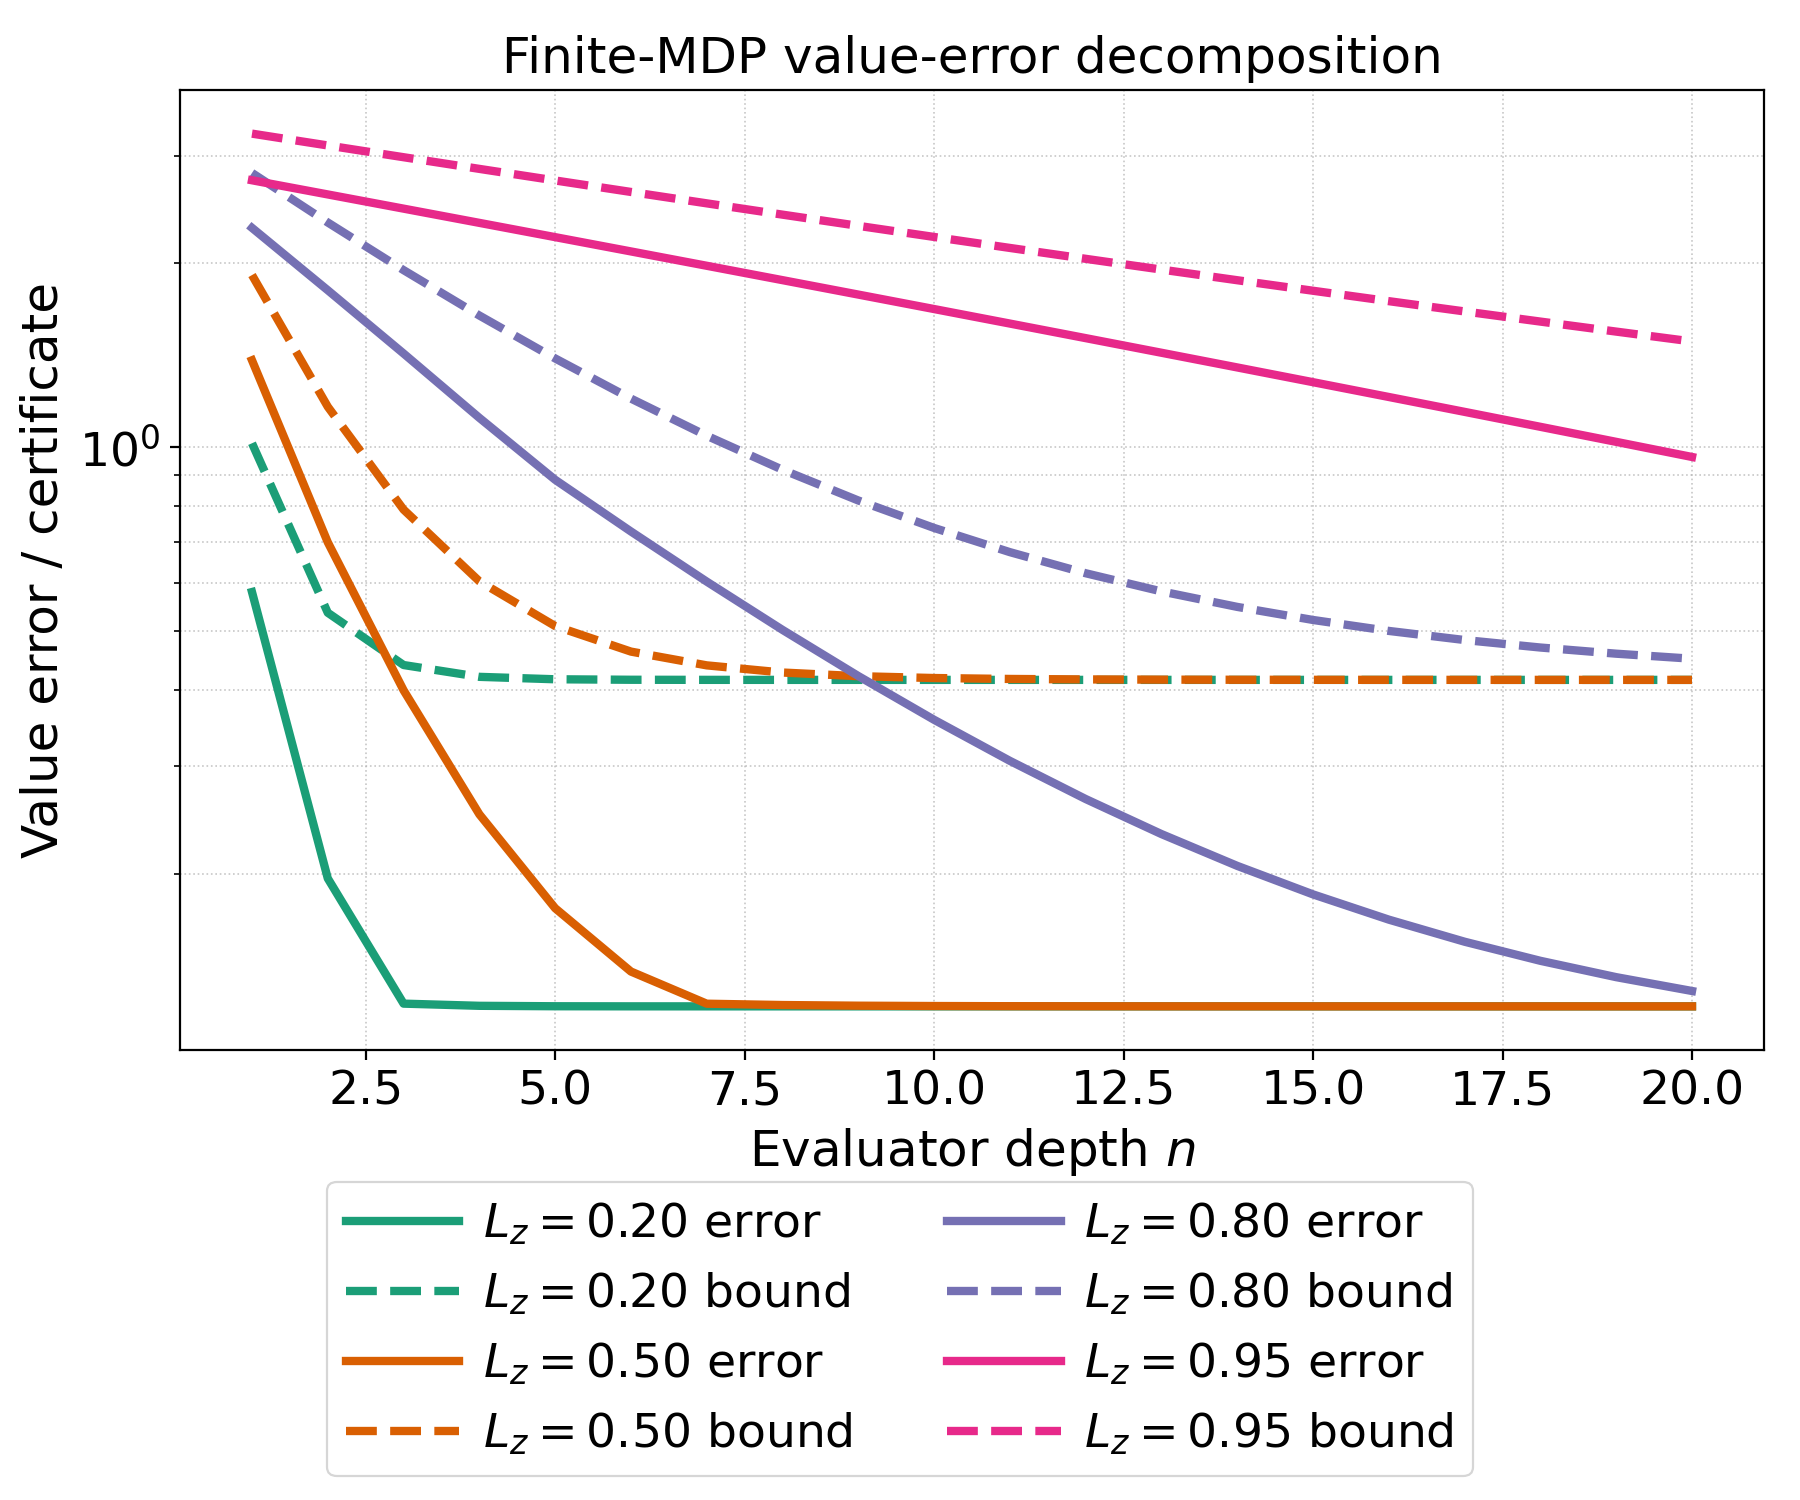
\includegraphics[width=\linewidth]{results/finite_mdp_certificate/fig_value_decomposition.png}
\caption{Value-error decomposition.}
\end{subfigure}\hfill
\begin{subfigure}[t]{0.48\textwidth}
\centering
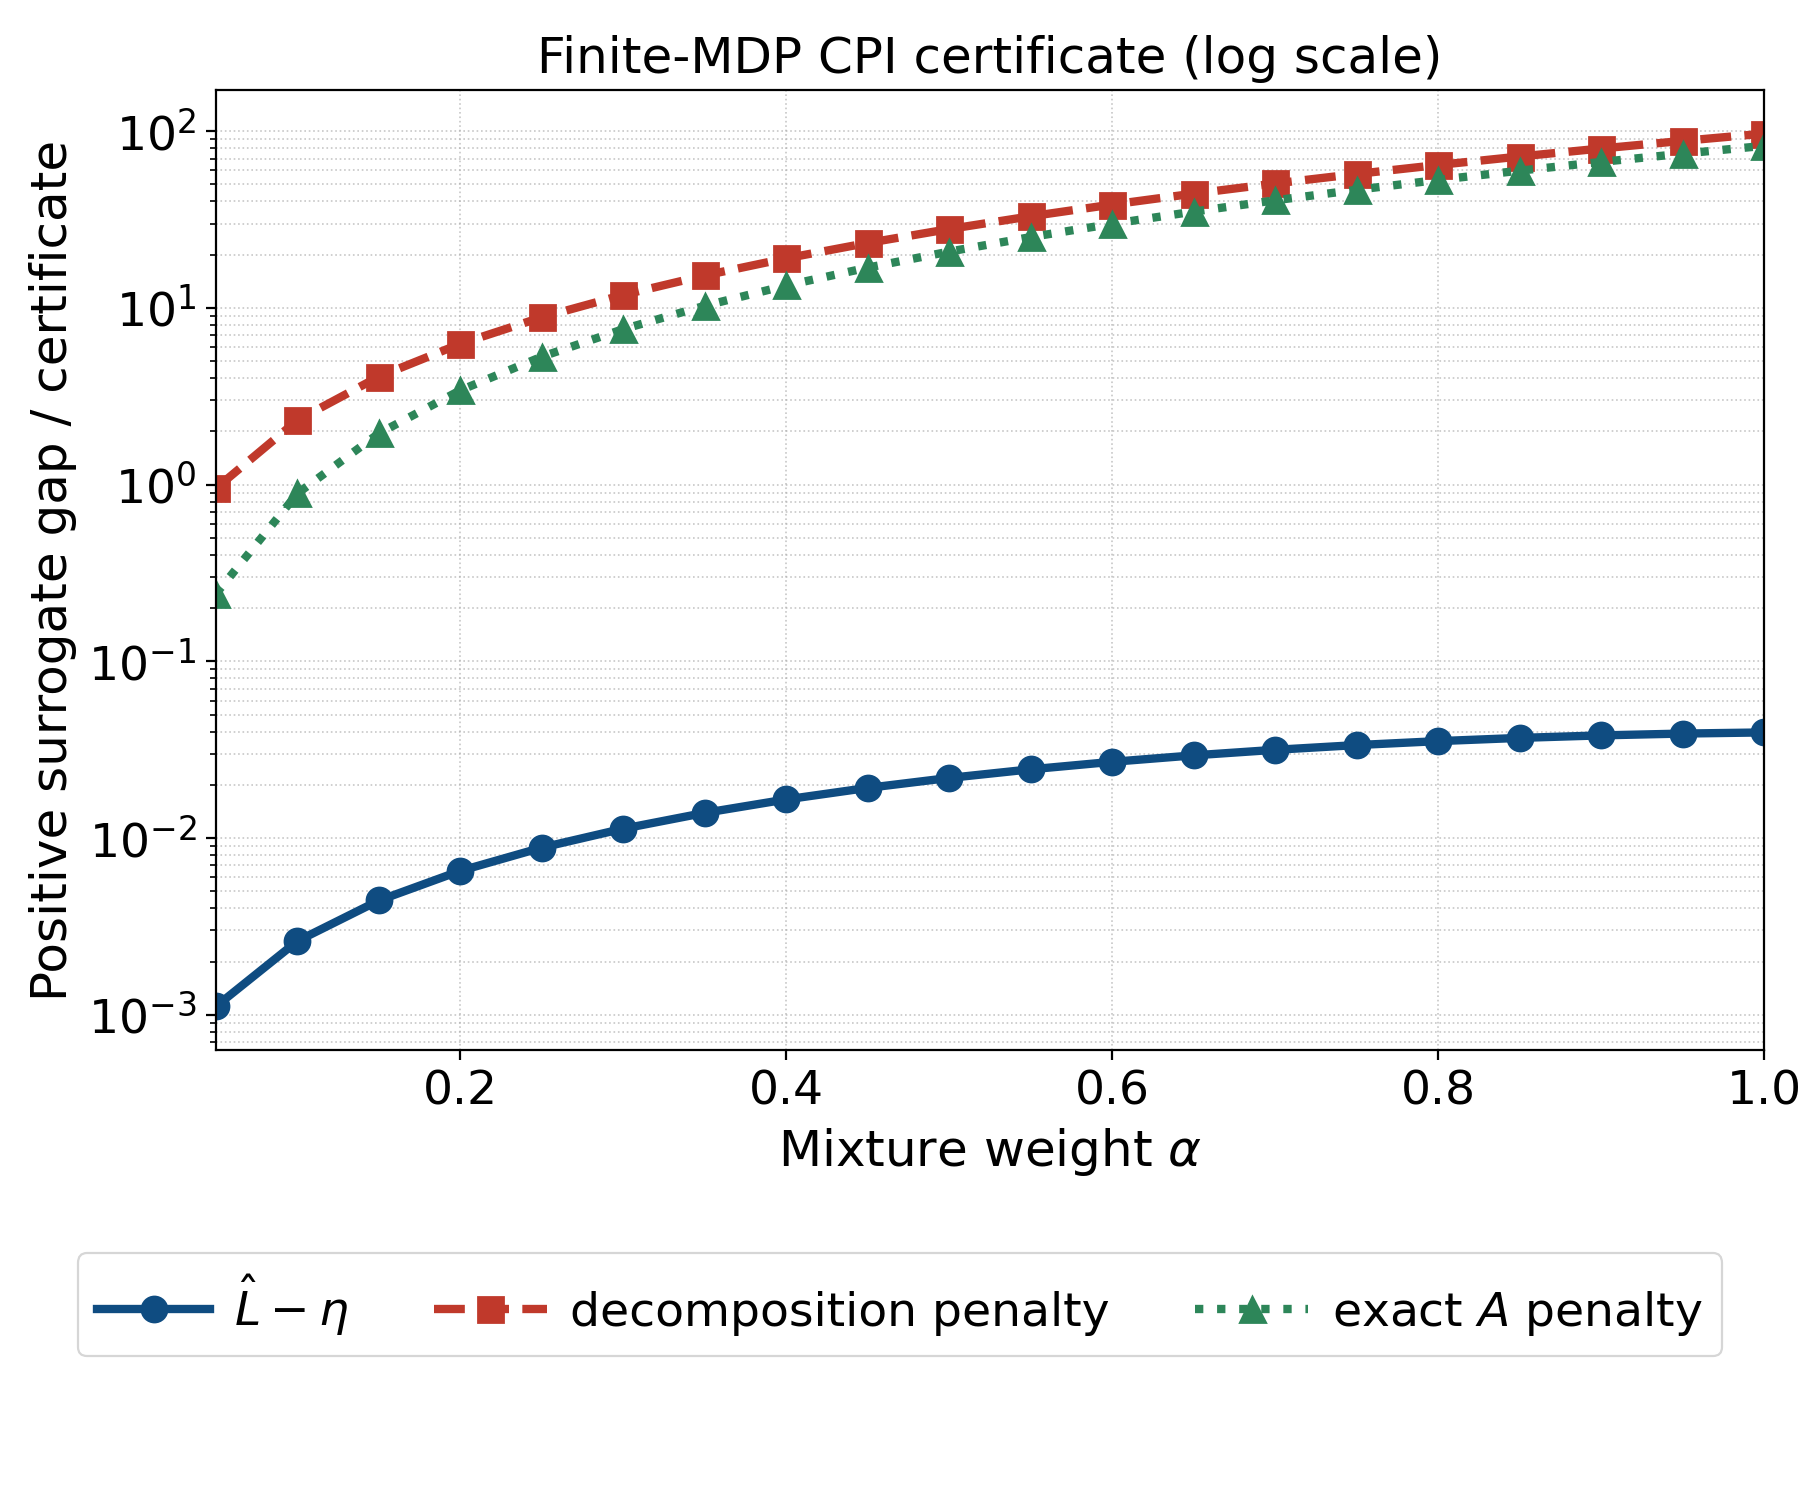
\includegraphics[width=\linewidth]{results/finite_mdp_certificate/fig_cpi_certificate.png}
\caption{CPI inequality check.}
\end{subfigure}
\caption{Finite-MDP theorem-pipeline unit test ($|\mathcal S|{=}64$, $|\mathcal A|{=}4$). Left: value error $\|U_n-V^\pi\|_\infty$ decays with evaluator depth $n$ and stays below the decomposition bound; larger $L_z$ slows the decay. Right: for $\pi_\alpha=(1-\alpha)\pi+\alpha\pi_{\mathrm{cand}}$, the surrogate gap (blue) stays below both the decomposition-based CPI penalty (red) and the tighter $\varepsilon_{A,\mathrm{cand}}$ penalty (green); log scale. All quantities are computed exactly by finite-state dynamic programming.}
\label{fig:finite_mdp_certificate_main}
\end{figure}

\begin{table}[t]
\caption{Compact definition of theorem-facing diagnostics. Each empirical value is batch-specific unless a uniform calculation is stated.}
\label{tab:diagnostics}
\centering
\small
\begin{tabularx}{\linewidth}{@{}llX@{}}
\toprule
Quantity & Appears in & Practical proxy / diagnostic \\
\midrule
$L_z^{\mathrm{pre/post}}$ & Assump.~\ref{ass:Lip} & Local finite-difference ratios before/after projection; not global moduli \\
$\rho_R$, active rate & Prop.~\ref{prop:proj_sat_contraction} & Batch minimum pre-projection norm and fraction with $\|f_\theta(z)\|>R$ \\
$C_z$, $L_V(R)$ & Assump.~\ref{ass:Lip} & Batch initial displacement and local finite-difference value-head ratio \\
$\|U_n-\mathcal T_K^\pi U_n\|$ & Remark~\ref{rem:residual_bridge} & $K$-step TD error on a declared diagnostic population \\
$\bar\varepsilon_{\mathrm{res},n}$ & Cor.~\ref{cor:persistent_cpi_augmented} & Augmented-state residual on a declared diagnostic population \\
$\varepsilon_{\mathrm{cent}}$ & Thm.~\ref{thm:monotone_with_error} & Statewise current-policy mean of $\widehat A$ \\
$\varepsilon_{A,\mathrm{cand}}$ & Thm.~\ref{thm:monotone_with_error} & Candidate-policy mean advantage error on declared states \\
TV / KL deployment gap & Thm.~\ref{thm:deployment_perturbation} & Exact mixture versus deployed-policy discrepancy on a declared recursive closure \\
\bottomrule
\end{tabularx}
\end{table}


\section{Notation Summary}
\label{app:notation}

We summarize notation here for convenience.
Table~\ref{tab:notation} lists additional symbols used in proofs.

\begin{table}[t]
\caption{Additional symbols and notations}
\label{tab:notation}
\begin{center}
\begin{tabular}{ll}
\toprule
Symbol & Meaning \\
\midrule
$h$, $\bar s=(x,y,z,h)$ & Remaining edit budget / clock-complete persistent state \\
$z^{(j)}(s)$, $U_j(s)$ & Latent and scalar value after finite depth $j$ \\
$U_*(s)$ & Fixed-point value used only in the contractive specialization \\
$B_{n,m}$ & Finite path/discrepancy plus depth-$m$ residual certificate \\
$\widetilde U_n(\bar s)$, $\widetilde U_*(\bar s)$ & Persistent finite-depth value / memoryless reference \\
$\varepsilon_{\mathrm{res},n}$ & Episodic finite-depth Bellman residual \\
$\bar\varepsilon_{\mathrm{res},n}$ & Persistent augmented-state finite-depth residual \\
$\bar\varepsilon_{\mathrm{res},*}$ & Augmented residual of the fixed-point reference \\
$L_{z^*}$, $\Delta y_{\max}$, $E_0$ & Slow-drift parameters \\
$\varepsilon_A$, $\bar\varepsilon_A$ & Episodic / augmented advantage error bounds \\
$\varepsilon_{\mathrm{res}}^*$ & Architectural residual at $U_*$ \\
$\varepsilon_{\mathrm{CPI}}$ & CPI constant \\
$\kappa_n = L_z^n$ & Contraction after $n$ steps \\
$\mathcal{R}_\Pi$ & Union of reachable sets for policy family $\Pi$ \\
$\supnorm{f}{\Pi}$ & Sup-norm over $\mathcal{R}_\Pi$ \\
$B_V(s)$ & Baseline: $\E_{b \sim \pi}[\widehat{Q}_V(s,b)]$ \\
\bottomrule
\end{tabular}
\end{center}
\end{table}

\section{Constructive Definition of the Advantage-Evaluation Closure}
\label{app:adv_closure_full}


\begin{definition}[Reachable set]
\label{def:reachable}
For a policy $\pi$ in a finite or countable MDP, let $\mathcal R_\pi$ be the exact set of states reached with positive probability under some state marginal $\rho P_\pi^t$, $t\ge0$, where $P_\pi$ is the policy-induced transition kernel.
\end{definition}

\begin{definition}[Advantage-evaluation closure]
\label{def:adv_closure}
Fix a current policy $\pi$ and a candidate policy $\pi_{\mathrm{cand}}$.
Let $\mathcal{R}_{\pi,\pi_{\mathrm{cand}}}^{\mathrm{adv}}$ contain $\mathcal R_\pi$ and $s_{\mathrm{abs}}$ such that
\begin{enumerate}
\item for every $s\in\mathcal R_\pi$ and every action in $\mathrm{supp}(\pi(\cdot|s))\cup\mathrm{supp}(\pi_{\mathrm{cand}}(\cdot|s))$, the next state lies in $\mathcal{R}_{\pi,\pi_{\mathrm{cand}}}^{\mathrm{adv}}$ almost surely; and
\item for every $s\in\mathcal{R}_{\pi,\pi_{\mathrm{cand}}}^{\mathrm{adv}}$ and $a\in\mathrm{supp}(\pi(\cdot|s))$, $P(\mathcal{R}_{\pi,\pi_{\mathrm{cand}}}^{\mathrm{adv}}\mid s,a)=1$.
\end{enumerate}
We write $\|f\|_{\infty,\pi,\pi_{\mathrm{cand}}}^{\mathrm{adv}}$ for the ordinary supremum of $|f|$ on this set, including the absorbing boundary.
\end{definition}


The following construction gives the exact closure in Definition~\ref{def:adv_closure}.

Fix a current policy $\pi$ and a candidate policy $\pi_{\mathrm{cand}}$.
Define the \emph{one-step deviation} set
\begin{equation}
\mathcal{R}_{\pi,\pi_{\mathrm{cand}}}^{+}
:=
\mathcal{R}_\pi
\;\cup\;
\bigl\{\,s' : \exists\, s\in\mathcal{R}_\pi,
\exists\, a\in \mathrm{supp}(\pi(\cdot|s))\cup\mathrm{supp}(\pi_{\mathrm{cand}}(\cdot|s))
\text{ with } P(s'\mid s,a)>0\,\bigr\}.
\label{eq:R_plus_def_app}
\end{equation}
Let $\mathcal{R}_{\pi,\pi_{\mathrm{cand}}}^{\mathrm{adv}}$ denote the smallest superset of $\mathcal{R}_{\pi,\pi_{\mathrm{cand}}}^{+}$ that is closed under forward dynamics of $\pi$:
\begin{align}
\mathcal{R}_{\pi,\pi_{\mathrm{cand}}}^{\mathrm{adv}}
&:=
\bigcup_{t\ge 0} \mathcal{R}^{(t)},
\qquad
\mathcal{R}^{(0)}=\mathcal{R}_{\pi,\pi_{\mathrm{cand}}}^{+},
\notag\\
\mathcal{R}^{(t+1)}&=\mathcal{R}^{(t)}\cup\{s' : \exists s\in \mathcal{R}^{(t)},\notag\\
&\qquad a\in \mathrm{supp}(\pi(\cdot|s)),\; P(s'\mid s,a)>0\}.
\label{eq:R_adv_def_app}
\end{align}
The sup-norm $\|f\|_{\infty,\pi,\pi_{\mathrm{cand}}}^{\mathrm{adv}}$ used throughout is the one introduced in Definition~\ref{def:adv_closure}.

\begin{remark}[Requirements for a general-kernel extension]
\label{rem:general_kernel_extension}
A general measurable-state-space extension is not part of the formal claims above. One route is to fix a single sigma-finite reference measure $\nu$ on the closure, with $\nu(\{s_{\mathrm{abs}}\})>0$, such that every relevant one-step transition law and every $K$-step $\pi$ transition law is absolutely continuous with respect to $\nu$. All essential suprema must then be taken in the same $L^\infty(\nu)$ space so that $\mathcal T_K^\pi$ is well defined on equivalence classes. For general action kernels, support conditions must be replaced by statements holding for $\pi(\cdot\mid s)$- and $\pi_{\mathrm{cand}}(\cdot\mid s)$-almost every action unless additional topology is specified. The CPI occupancy argument must likewise be written for finite signed measures in total variation rather than for probability vectors in $\ell_1$.
\end{remark}

\section{Shaping Convention and Absorbing-State Normalization}
\label{app:shaping_convention}

We use potential-based shaping with potential $\Phi(s)=c(x,y)$ for episodic $s=(x,y,h)$ and persistent $\bar s=(x,y,z,h)$ (the potential ignores the clock and latent), and $\Phi(s_{\mathrm{abs}})=C_{\max}$ on their shared absorbing atom. We define
\begin{equation}
r(s,a,s')
=
r_0(s,a,s')
+
\gamma\,\Phi(s')-\Phi(s),
\end{equation}
applying shaping on \emph{all} transitions, including the absorbing self-loop.

For the absorbing self-loop, taking $r_0(s_{\mathrm{abs}},a,s_{\mathrm{abs}})=0$ gives
\[
r(s_{\mathrm{abs}},a,s_{\mathrm{abs}})
=
\gamma \Phi(s_{\mathrm{abs}})-\Phi(s_{\mathrm{abs}})
=
(\gamma-1)C_{\max}.
\]
Thus every policy satisfies the fixed shaped boundary value
\[
V^\pi(s_{\mathrm{abs}})
=
\sum_{t=0}^\infty \gamma^t (\gamma-1)C_{\max}
=
-C_{\max}.
\]

If one prefers the standard normalization $V(s_{\mathrm{abs}})=0$, use the shifted potential
$\tilde{\Phi}(s):=\Phi(s)-C_{\max}$.
This adds the constant reward $(1-\gamma)C_{\max}$ to every transition and shifts all returns by $+C_{\max}$ independently of the policy.
Accordingly, performance differences and optimal policies are unchanged.

\section{Finite-Horizon and Deployment-Aware Bounds}
\label{app:finite_horizon_extensions}

This section uses the finite edit clock directly. All statements are for
finite or countable state and action spaces and ordinary suprema. Fix
$0\le\gamma<1$, an integer horizon $H\ge0$, and one shared absorbing atom with
value
\[
b:=V^\pi(s_{\mathrm{abs}})=-C_{\max},
\qquad
r_{\mathrm{abs}}=(1-\gamma)b.
\]
Thus $b=r_{\mathrm{abs}}+\gamma b$. Every reward interval below includes
$r_{\mathrm{abs}}$.

For each $h\in\{1,\ldots,H\}$, let $\mathcal R_h$ be a finite or countable
clock-complete nonabsorbing stage closure. A transition from stage $h$ enters
$\mathcal R_{h-1}$ or $s_{\mathrm{abs}}$, and a stage-$1$ transition is
absorbing. The closure contains the current-policy reachable states, every
one-deviation successor for actions supported by the current or candidate
policy, and every recursive current-policy successor needed by the backups
below. In particular, it is forward invariant under those stage kernels. For
$1\le\ell\le h$, define
\begin{align}
(\mathcal T_{h:\ell}^{\pi}W)(s)
&:=\E\!\left[
\sum_{i=0}^{\ell-1}\gamma^i r_i
+\gamma^\ell W(S_\ell)
\mid S_0=s,\ A_i\sim\pi
\right],
\label{eq:fh_stage_operator}
\end{align}
where an absorbed trajectory remains at the shared atom and
$W(s_{\mathrm{abs}})=b$. Truncating when the clock reaches zero is therefore
equivalent to padding a longer backup with absorbing self-loops.

\begin{theorem}[Finite-horizon residual and finite-reference bound]
\label{thm:finite_horizon_reference}
Fix $0\le\gamma<1$, $H\ge0$, and $K\ge1$. Assume the finite or countable
stage closures contain the current-policy reachable states, the one-deviation
successors of every action supported by the current or candidate policy, and
all recursive current-policy successors used by $\mathcal T_{h:\ell}^{\pi}$.
Fix one frozen recurrent map $F$, a common initialization
$z_h^{(0)}(s)=z_{\mathrm{init}}(s)$, one latent norm, and one bounded scalar
head $V_\psi$. For every depth $q\ge0$, use the common construction
\[
z_h^{(q+1)}(s)=F(z_h^{(q)}(s),s),
\qquad
U_{h,q}(s)=V_\psi(z_h^{(q)}(s),x),
\]
and assign $U_{h,q}(s_{\mathrm{abs}})=b$ for every $h$ and $q$. The true
stage value has the same boundary, $V_h^\pi(s_{\mathrm{abs}})=b$, and all
displayed functions and rewards are bounded on the recursive closure. For
$h\ge1$, let
\begin{align}
\ell_h&:=\min\{K,h\},
&J_h&:=\left\lceil\frac{h}{K}\right\rceil,
\notag\\
\epsilon_{h,m}
&:=\left\|U_{h,m}
-\mathcal T_{h:\ell_h}^{\pi}U_{h-\ell_h,m}\right\|_{\infty,h},
&D_{h;n,m}&:=\|U_{h,n}-U_{h,m}\|_{\infty,h},
\label{eq:fh_residual_def}
\end{align}
where $U_{0,m}=b$. Then, for finite depths $0\le n<m$,
\begin{align}
\|U_{h,n}-V_h^\pi\|_{\infty,h}
&\le D_{h;n,m}
+\sum_{j=0}^{J_h-1}\gamma^{jK}\epsilon_{h-jK,m}.
\label{eq:fh_finite_reference}
\end{align}
Consequently, with
$\epsilon_m^{(h)}:=\max_{1\le r\le h}\epsilon_{r,m}$,
\begin{align}
\|U_{h,n}-V_h^\pi\|_{\infty,h}
&\le D_{h;n,m}
+\frac{1-\gamma^{KJ_h}}{1-\gamma^K}\epsilon_m^{(h)}.
\label{eq:fh_finite_reference_uniform}
\end{align}
If $V_\psi$ is $L_V$-Lipschitz in the common latent norm, then
\begin{align}
D_{h;n,m}
&\le L_V\sum_{q=n}^{m-1}
\sup_{s\in\mathcal R_h}
\|z_h^{(q+1)}(s)-z_h^{(q)}(s)\|.
\label{eq:fh_path_bound}
\end{align}
For $h=0$, set $J_0=0$; every sum is empty and the error is zero. In a
persistent-state application, $s=(x,y,z,h)$ and both policy kernels must use
the same frozen recurrent map that determines the carried-latent transition.
\end{theorem}

\begin{proof}
Write $e_{h,m}:=\|U_{h,m}-V_h^\pi\|_{\infty,h}$ and $e_{0,m}=0$. Since
$V_h^\pi=\mathcal T_{h:\ell_h}^\pi V_{h-\ell_h}^\pi$, the triangle inequality
and the stage-operator contraction give
\begin{align*}
e_{h,m}
&\le \epsilon_{h,m}
+\left\|\mathcal T_{h:\ell_h}^\pi U_{h-\ell_h,m}
-\mathcal T_{h:\ell_h}^\pi V_{h-\ell_h}^\pi\right\|_{\infty,h}\\
&\le \epsilon_{h,m}+\gamma^{\ell_h}e_{h-\ell_h,m}.
\end{align*}
On paths absorbed inside the block, the terminal-function difference is zero
because both functions equal $b$. Unrolling the recursion yields residuals at
clocks $h,h-K,\ldots,h-(J_h-1)K$ with weights
$1,\gamma^K,\ldots,\gamma^{(J_h-1)K}$. The final partial block multiplies
$e_{0,m}=0$, proving the residual sum. Bounding every residual by
$\epsilon_m^{(h)}$ gives the geometric factor. Adding and subtracting
$U_{h,m}$ proves Eqs.~\eqref{eq:fh_finite_reference}--
\eqref{eq:fh_finite_reference_uniform}. Finally, Lipschitzness and telescoping
the common recurrent path from depth $n$ to $m$ prove
Eq.~\eqref{eq:fh_path_bound}.
\end{proof}

The next result uses the exact finite-horizon performance
\[
\eta_H(\pi):=\E\!\left[
\sum_{t=0}^{H-1}\gamma^t r_t+\gamma^H b
\right],
\]
where early terminal trajectories are padded by the absorbing self-loop. Let
$d_t^\pi$ be the probability law before decision $t$, including absorbed
mass, and define every advantage to be zero at the absorbing atom.

\begin{theorem}[Finite-horizon CPI with centered evaluation error]
\label{thm:finite_horizon_cpi}
Fix $0\le\gamma<1$, $H\ge0$, bounded rewards, and the exact common terminal
boundary $b$. Fix a current stage policy $\pi_h$, a candidate
$\pi_{\mathrm{cand},h}$, and
the exact pointwise mixture
\[
\pi_{\alpha,h}=(1-\alpha)\pi_h
+\alpha\pi_{\mathrm{cand},h},
\qquad \alpha\in[0,1].
\]
All three policies act in the same fixed time-indexed MDP. Their finite or
countable recursive stage closure contains the complete support of $d_t^\pi$
and $d_t^{\pi_\alpha}$ for every $t$, the one-step successors of actions
supported by $\pi_h$ or $\pi_{\mathrm{cand},h}$, and all later successors
needed by both occupancy laws. Define
\begin{align}
\delta_h(s)
&:=\E_{a\sim\pi_{\mathrm{cand},h}(\cdot\mid s)}[A_h^\pi(s,a)],
&\epsilon_{\mathrm{CPI},h}&:=\sup_s|\delta_h(s)|.
\label{eq:fh_cpi_delta}
\end{align}
Let $\widehat A_h$ be exactly statewise centered under the current policy,
\begin{align}
\E_{a\sim\pi_h(\cdot\mid s)}[\widehat A_h(s,a)]&=0,
\label{eq:fh_centering}
\end{align}
and let the finite candidate-policy bias be
\begin{align}
\epsilon_{A,\mathrm{cand},h}
&:=\sup_s\left|
\E_{a\sim\pi_{\mathrm{cand},h}(\cdot\mid s)}
[\widehat A_h(s,a)-A_h^\pi(s,a)]
\right|.
\label{eq:fh_candidate_bias}
\end{align}
Define the estimated surrogate
\begin{align}
\widehat L_{H,\pi}(\pi_\alpha)
&:=\eta_H(\pi)+\sum_{t=0}^{H-1}\gamma^t
\E_{\substack{s\sim d_t^\pi,\\
a\sim\pi_{\alpha,H-t}(\cdot\mid s)}}
[\widehat A_{H-t}(s,a)].
\label{eq:fh_estimated_surrogate}
\end{align}
Then
\begin{align}
\eta_H(\pi_\alpha)
\ge{}&\widehat L_{H,\pi}(\pi_\alpha)
-\alpha\sum_{t=0}^{H-1}\gamma^t
\epsilon_{A,\mathrm{cand},H-t}
\notag\\
&-2\alpha\sum_{t=0}^{H-1}\gamma^t
\epsilon_{\mathrm{CPI},H-t}[1-(1-\alpha)^t].
\label{eq:fh_cpi_exact_coupling}
\end{align}
Using $1-(1-\alpha)^t\le\alpha t$ gives
\begin{align}
\eta_H(\pi_\alpha)
\ge{}&\widehat L_{H,\pi}(\pi_\alpha)
-\alpha\sum_{t=0}^{H-1}\gamma^t
\epsilon_{A,\mathrm{cand},H-t}
-2\alpha^2\sum_{t=0}^{H-1}t\gamma^t
\epsilon_{\mathrm{CPI},H-t}.
\label{eq:fh_cpi_quadratic}
\end{align}
For uniform bounds $\epsilon_{A,\mathrm{cand},h}\le
\epsilon_{A,\mathrm{cand}}$ and
$\epsilon_{\mathrm{CPI},h}\le\epsilon_{\mathrm{CPI}}$, set
\begin{align}
G_H(q)&:=\sum_{t=0}^{H-1}q^t=\frac{1-q^H}{1-q},
&S_H(\gamma)&:=\sum_{t=0}^{H-1}t\gamma^t.
\label{eq:fh_GS_def}
\end{align}
The two penalties become, respectively,
\begin{align}
&\alpha\epsilon_{A,\mathrm{cand}}G_H(\gamma)
+2\alpha\epsilon_{\mathrm{CPI}}
[G_H(\gamma)-G_H(\gamma(1-\alpha))],
\label{eq:fh_cpi_uniform_exact}\\
&\alpha\epsilon_{A,\mathrm{cand}}G_H(\gamma)
+2\alpha^2\epsilon_{\mathrm{CPI}}S_H(\gamma).
\label{eq:fh_cpi_uniform_quadratic}
\end{align}
For $H=0$, define $G_0=S_0=0$; the policies have identical performance and
all penalties vanish.
\end{theorem}

\begin{proof}
The time-indexed performance-difference identity is
\begin{align}
\eta_H(\pi_\alpha)-\eta_H(\pi)
&=\alpha\sum_{t=0}^{H-1}\gamma^t
\E_{s\sim d_t^{\pi_\alpha}}[\delta_{H-t}(s)].
\label{eq:fh_performance_difference}
\end{align}
It follows by telescoping the stage Bellman equations; the terminal term
cancels because both policies use $b$. Couple the exact mixture with the
current policy while the two trajectories share a state. With probability
$1-\alpha$, choose the current-policy component and use the same action and
transition randomness. Thus
\begin{align}
\|d_t^{\pi_\alpha}-d_t^\pi\|_1
&\le2[1-(1-\alpha)^t]\le2\alpha t.
\label{eq:fh_occupancy_coupling}
\end{align}
Replacing $d_t^{\pi_\alpha}$ by $d_t^\pi$ in
Eq.~\eqref{eq:fh_performance_difference} therefore incurs at most the final
term of Eq.~\eqref{eq:fh_cpi_exact_coupling}. Exact centering eliminates the
current-policy component of
$\E_{a\sim\pi_{\alpha,h}}[A_h^\pi-\widehat A_h]$ pointwise. The remaining
candidate component is bounded by
$\alpha\epsilon_{A,\mathrm{cand},h}$, proving the first penalty and
Eq.~\eqref{eq:fh_cpi_exact_coupling}. The union bound in
Eq.~\eqref{eq:fh_occupancy_coupling} proves
Eq.~\eqref{eq:fh_cpi_quadratic}. Summing the two geometric series gives
Eqs.~\eqref{eq:fh_cpi_uniform_exact}--
\eqref{eq:fh_cpi_uniform_quadratic}. Empty sums prove the $H=0$ case.
\end{proof}

\begin{theorem}[Deployment perturbation from the exact mixture]
\label{thm:deployment_perturbation}
Fix $0\le\gamma<1$. Let
$\pi_\alpha=(1-\alpha)\pi+\alpha\pi_{\mathrm{cand}}$ be the exact mixture
and let $\widetilde\pi$ be the deployed policy in the same fixed MDP. Let
$\mathcal D$ be either the full state space or a closure containing the
initial-law support that is recursively forward invariant under both policies.
For every $s\in\mathcal D$, define
\[
\mathcal A_{\mathcal D}(s)
:=\operatorname{supp}\pi_\alpha(\cdot\mid s)
\cup\operatorname{supp}\widetilde\pi(\cdot\mid s),
\]
and require $\mathcal D$ to contain every one-step successor of every action
in $\mathcal A_{\mathcal D}(s)$, including states reachable only through
deployed-policy support. Suppose all such transition rewards, including the
absorbing self-loop, lie in $[r_{\min},r_{\max}]$, and write
$\Delta_r=r_{\max}-r_{\min}$. If
\begin{align}
\sup_{s\in\mathcal D}
\operatorname{TV}(\widetilde\pi(\cdot\mid s),
\pi_\alpha(\cdot\mid s))&\le\delta,
\label{eq:deployment_uniform_tv}
\end{align}
then
\begin{align}
|\eta(\widetilde\pi)-\eta(\pi_\alpha)|
&\le\frac{\Delta_r\delta}{(1-\gamma)^2}
\le\frac{2R_{\max}\delta}{(1-\gamma)^2}
\quad\text{when }|r|\le R_{\max}.
\label{eq:deployment_tv_bound}
\end{align}
For a horizon $H$, assume corresponding stage domains $\mathcal D_h$ are
recursively invariant under both policies, use one exact terminal boundary
$b$, and impose Eq.~\eqref{eq:deployment_uniform_tv} uniformly over all
stages. Then
\begin{align}
|\eta_H(\widetilde\pi)-\eta_H(\pi_\alpha)|
&\le\Delta_r\delta\sum_{t=0}^{H-1}
\gamma^tG_{H-t}(\gamma)
\notag\\
&=\frac{\Delta_r\delta}{1-\gamma}
[G_H(\gamma)-H\gamma^H].
\label{eq:deployment_tv_finite_horizon}
\end{align}
The finite-horizon right-hand side is zero for $H=0$. If the state is the
persistent augmented state $(x,y,z,h)$, both policies must share the frozen
recurrent map that determines the carried-latent transition; changing it would
change the MDP and is outside this theorem.
\end{theorem}

\begin{proof}
For the exact-mixture action value,
\begin{align*}
\operatorname{osc}_{a\in\mathcal A_{\mathcal D}(s)}
Q^{\pi_\alpha}(s,a)
&\le\frac{\Delta_r}{1-\gamma}.
\end{align*}
The total-variation expectation inequality and
$\E_{a\sim\pi_\alpha}A^{\pi_\alpha}(s,a)=0$ give
\[
\left|\E_{a\sim\widetilde\pi}
A^{\pi_\alpha}(s,a)\right|
\le\frac{\Delta_r\delta}{1-\gamma}.
\]
The performance-difference identity under $\widetilde\pi$ proves
Eq.~\eqref{eq:deployment_tv_bound}. With $h$ decisions left, the common
terminal boundary cancels and
$\operatorname{osc}_a Q_h^{\pi_\alpha}\le\Delta_r G_h(\gamma)$. Summing the
time-indexed performance-difference identity gives the first line of
Eq.~\eqref{eq:deployment_tv_finite_horizon}; expanding $G_{H-t}$ gives its
closed form. The empty sum gives the $H=0$ case.
\end{proof}

\begin{corollary}[Either-direction uniform-KL deployment bound]
\label{cor:deployment_pinsker}
Under Theorem~\ref{thm:deployment_perturbation}, suppose either
\begin{align*}
\sup_{s\in\mathcal D}
D_{\mathrm{KL}}(\widetilde\pi(\cdot\mid s)\|\pi_\alpha(\cdot\mid s))
&\le\kappa,
\quad\text{or}\\
\sup_{s\in\mathcal D}
D_{\mathrm{KL}}(\pi_\alpha(\cdot\mid s)\|\widetilde\pi(\cdot\mid s))
&\le\kappa,
\end{align*}
for a finite $\kappa$. Then Pinsker's inequality gives
$\delta\le\sqrt{\kappa/2}$, so
\begin{align}
|\eta(\widetilde\pi)-\eta(\pi_\alpha)|
&\le\frac{\Delta_r}{(1-\gamma)^2}\sqrt{\frac{\kappa}{2}}.
\label{eq:deployment_kl_bound}
\end{align}
The same substitution in Eq.~\eqref{eq:deployment_tv_finite_horizon} gives
the finite-horizon corollary. If the selected KL direction is infinite because
the supports are incompatible, no finite Pinsker bound follows; the TV result
remains available if Eq.~\eqref{eq:deployment_uniform_tv} is established.
\end{corollary}

\begin{proof}
Pinsker's inequality in either stated direction bounds the symmetric total
variation distance by $\sqrt{\kappa/2}$. Substitute this value for $\delta$ in
Eqs.~\eqref{eq:deployment_tv_bound} and
\eqref{eq:deployment_tv_finite_horizon}.
\end{proof}

\begin{remark}[Uniform assumptions versus finite-batch diagnostics]
\label{rem:deployment_uniform_scope}
The residual, centering, TV, and KL conditions above are uniform on their
declared recursive closures. A replay-batch mean, batch maximum, held-out
finite maximum, or local finite-difference proxy is only a finite-batch
diagnostic and does not instantiate these theorems. No retained historical
checkpoint is claimed to satisfy the new conditions.
\end{remark}

\section{CPI Derivation for Mixture Policies}
\label{app:cpi_derivation}

We derive the CPI bound~\eqref{eq:cpi_bound} specialized to mixture policies $\pi_{\mathrm{new}} = (1-\alpha)\pi + \alpha\pi_{\mathrm{cand}}$, following the framework of~\citet{KakadeLangford2002}.

This derivation is stated for finite or countable state and action spaces, where discounted occupancies are probability mass functions and $\|\cdot\|_1$ has its usual meaning. A general-kernel extension requires the total-variation formulation and common-domination conditions in Remark~\ref{rem:general_kernel_extension}.

\textbf{Setup.}
Define the \emph{advantage function under the greedy policy $\pi_{\mathrm{cand}}$}:
\begin{equation}
\delta(s) := \E_{a \sim \pi_{\mathrm{cand}}(\cdot|s)}[A^\pi(s,a)].
\end{equation}
Note that $|\delta(s)| \le \varepsilon_{\mathrm{CPI}} := \sup_s |\delta(s)|$ by definition.

For the mixture policy $\pi_{\mathrm{new}} = (1-\alpha)\pi + \alpha\pi_{\mathrm{cand}}$:
\begin{align}
\E_{a \sim \pi_{\mathrm{new}}(\cdot|s)}[A^\pi(s,a)]
&= (1-\alpha)\underbrace{\E_{a \sim \pi}[A^\pi(s,a)]}_{=0} + \alpha \E_{a \sim \pi_{\mathrm{cand}}}[A^\pi(s,a)] \\
&= \alpha \delta(s).
\end{align}
\textbf{Action-set convention.}
If the available edit actions depend on the plan (and hence on the state $s=(x,y,h)$), we interpret $\pi(\cdot\mid s)$ and
$\pi_{\mathrm{cand}}(\cdot\mid s)$ as distributions on the same per-state action set $\AAcal(s)$.
Equivalently, we may embed both policies into a fixed superset action space by assigning probability $0$ to invalid actions.
Under either convention, $\|\pi'(\cdot\mid s)-\pi(\cdot\mid s)\|_1\le 2$ holds for all $s$.
\textbf{Performance difference lemma.}
The standard performance difference lemma~\citep{KakadeLangford2002} gives:
\begin{equation}
\eta(\pi_{\mathrm{new}}) - \eta(\pi) = \frac{1}{1-\gamma} \E_{s \sim d_{\pi_{\mathrm{new}}}}[\E_{a \sim \pi_{\mathrm{new}}}[A^\pi(s,a)]] = \frac{\alpha}{1-\gamma} \E_{s \sim d_{\pi_{\mathrm{new}}}}[\delta(s)].
\end{equation}

\textbf{Distribution shift bound.}
We need to relate $\E_{s \sim d_{\pi_{\mathrm{new}}}}[\delta(s)]$ to $\E_{s \sim d_\pi}[\delta(s)]$.
The key is to bound $\|d_{\pi_{\mathrm{new}}} - d_\pi\|_1$.

\begin{lemma}[Occupancy measure coupling]
\label{lem:occupancy_coupling}
For any two policies $\pi'$ and $\pi$ in an MDP with discount $\gamma$:
\begin{equation}
\|d_{\pi'} - d_\pi\|_1 \le \frac{\gamma}{1-\gamma} \E_{s \sim d_{\pi'}}[\|\pi'(\cdot|s) - \pi(\cdot|s)\|_1].
\end{equation}
\end{lemma}

\begin{proof}
Recall the discounted occupancy satisfies the fixed-point equation
\[
d_\pi = (1-\gamma)\rho + \gamma\, d_\pi P_\pi,
\qquad
d_{\pi'} = (1-\gamma)\rho + \gamma\, d_{\pi'} P_{\pi'}.
\]
Subtracting gives
\[
d_{\pi'}-d_\pi
=
\gamma\bigl(d_{\pi'}P_{\pi'}-d_\pi P_\pi\bigr)
=
\gamma\bigl(d_{\pi'}(P_{\pi'}-P_\pi) + (d_{\pi'}-d_\pi)P_\pi\bigr).
\]
Taking $\ell_1$ norms and using that $P_\pi$ is a Markov operator (so it is non-expansive in $\ell_1$),
\[
\|d_{\pi'}-d_\pi\|_1
\le
\gamma\|d_{\pi'}(P_{\pi'}-P_\pi)\|_1
+\gamma\|(d_{\pi'}-d_\pi)P_\pi\|_1
\le
\gamma\|d_{\pi'}(P_{\pi'}-P_\pi)\|_1
+\gamma\|d_{\pi'}-d_\pi\|_1.
\]
Rearranging yields
\[
\|d_{\pi'}-d_\pi\|_1
\le
\frac{\gamma}{1-\gamma}\,\|d_{\pi'}(P_{\pi'}-P_\pi)\|_1.
\]
Finally,
\begin{align}
\|d_{\pi'}(P_{\pi'}-P_\pi)\|_1
&=
\Bigl\|
\sum_s d_{\pi'}(s)\bigl(P_{\pi'}(\cdot|s)-P_\pi(\cdot|s)\bigr)
\Bigr\|_1
\notag\\
&\le
\sum_s d_{\pi'}(s)\,\bigl\|P_{\pi'}(\cdot|s)-P_\pi(\cdot|s)\bigr\|_1
\notag\\
&=
\E_{s\sim d_{\pi'}}\bigl[\|P_{\pi'}(\cdot|s)-P_\pi(\cdot|s)\|_1\bigr]
\notag\\
&=
\E_{s\sim d_{\pi'}}\Bigl[\Bigl\|\sum_a \bigl(\pi'(a|s)-\pi(a|s)\bigr)\,P(\cdot\mid s,a)\Bigr\|_1\Bigr]
\notag\\
&\le
\E_{s\sim d_{\pi'}}\Bigl[\sum_a \bigl|\pi'(a|s)-\pi(a|s)\bigr|\,\underbrace{\|P(\cdot\mid s,a)\|_1}_{=1}\Bigr]
\notag\\
&=
\E_{s\sim d_{\pi'}}\bigl[\|\pi'(\cdot|s)-\pi(\cdot|s)\|_1\bigr],
\end{align}
which gives the claim.
\end{proof}

For our mixture:
\begin{equation}
\|\pi_{\mathrm{new}}(\cdot|s) - \pi(\cdot|s)\|_1
=
\alpha \|\pi_{\mathrm{cand}}(\cdot|s) - \pi(\cdot|s)\|_1
\le 2\alpha,
\end{equation}
since $\|p-q\|_1\le 2$ for any two probability distributions $p,q$ on the same action space.


Thus:
\begin{equation}
\|d_{\pi_{\mathrm{new}}} - d_\pi\|_1 \le \frac{2\gamma\alpha}{1-\gamma}.
\end{equation}

\textbf{Combining the bounds.}
Write:
\begin{align}
\E_{s \sim d_{\pi_{\mathrm{new}}}}[\delta(s)] &= \E_{s \sim d_\pi}[\delta(s)] + \left(\E_{s \sim d_{\pi_{\mathrm{new}}}}[\delta(s)] - \E_{s \sim d_\pi}[\delta(s)]\right).
\end{align}

The second term is bounded by:
\begin{equation}
\left|\E_{s \sim d_{\pi_{\mathrm{new}}}}[\delta(s)] - \E_{s \sim d_\pi}[\delta(s)]\right| \le \|d_{\pi_{\mathrm{new}}} - d_\pi\|_1 \cdot \sup_s|\delta(s)| \le \frac{2\gamma\alpha}{1-\gamma} \varepsilon_{\mathrm{CPI}}.
\end{equation}

Therefore:
\begin{align}
\eta(\pi_{\mathrm{new}}) &= \eta(\pi) + \frac{\alpha}{1-\gamma} \E_{s \sim d_{\pi_{\mathrm{new}}}}[\delta(s)] \\
&\ge \eta(\pi) + \frac{\alpha}{1-\gamma} \E_{s \sim d_\pi}[\delta(s)] - \frac{\alpha}{1-\gamma} \cdot \frac{2\gamma\alpha}{1-\gamma} \varepsilon_{\mathrm{CPI}} \\
&= L_\pi(\pi_{\mathrm{new}}) - \frac{2\gamma\varepsilon_{\mathrm{CPI}}}{(1-\gamma)^2} \alpha^2,
\end{align}
where in the last step we used $L_\pi(\pi_{\mathrm{new}}) = \eta(\pi) + \frac{1}{1-\gamma}\E_{s \sim d_\pi, a \sim \pi_{\mathrm{new}}}[A^\pi(s,a)] = \eta(\pi) + \frac{\alpha}{1-\gamma}\E_{s \sim d_\pi}[\delta(s)]$.

This establishes~\eqref{eq:cpi_bound}.

\begin{corollary}[CPI with a centering defect]
\label{cor:cpi_centering_defect}
Use the setup of Theorem~\ref{thm:monotone_with_error}, but replace the exact-centering condition~\eqref{eq:centering_condition} by
\[
\varepsilon_{\mathrm{cent}}
:=
\sup_{s\in\mathcal R_\pi}
\left|
\E_{a\sim\pi(\cdot\mid s)}[\widehat A(s,a)]
\right|
<\infty.
\]
Then
\begin{equation}
\eta(\pi_{\mathrm{new}})
\ge
\widehat L_\pi(\pi_{\mathrm{new}})
-
\frac{(1-\alpha)\varepsilon_{\mathrm{cent}}+\alpha\varepsilon_{A,\mathrm{cand}}}{1-\gamma}
-
\frac{2\varepsilon_{\mathrm{CPI}}\gamma}{(1-\gamma)^2}\alpha^2.
\label{eq:cpi_centering_defect_bound}
\end{equation}
\end{corollary}

\begin{proof}
The CPI shell gives
\[
\eta(\pi_{\mathrm{new}})
\ge
L_\pi(\pi_{\mathrm{new}})
-
\frac{2\varepsilon_{\mathrm{CPI}}\gamma}{(1-\gamma)^2}\alpha^2.
\]
For each $s\in\mathcal R_\pi$,
\begin{align*}
&\E_{a\sim\pi_{\mathrm{new}}(\cdot\mid s)}
[A^\pi(s,a)-\widehat A(s,a)] \\
&=
(1-\alpha)
\E_{a\sim\pi(\cdot\mid s)}
[A^\pi(s,a)-\widehat A(s,a)]
+
\alpha
\E_{a\sim\pi_{\mathrm{cand}}(\cdot\mid s)}
[A^\pi(s,a)-\widehat A(s,a)].
\end{align*}
Since $\E_{a\sim\pi}[A^\pi(s,a)]=0$, the first term is bounded below by
$-(1-\alpha)\varepsilon_{\mathrm{cent}}$.
By the definition of $\varepsilon_{A,\mathrm{cand}}$, the second term is bounded below by
$-\alpha\varepsilon_{A,\mathrm{cand}}$.
Therefore
\[
L_\pi(\pi_{\mathrm{new}})
\ge
\widehat L_\pi(\pi_{\mathrm{new}})
-
\frac{(1-\alpha)\varepsilon_{\mathrm{cent}}+\alpha\varepsilon_{A,\mathrm{cand}}}{1-\gamma}.
\]
Combining the two displays proves~\eqref{eq:cpi_centering_defect_bound}.
\end{proof}

\subsection{Proof of Corollary~\ref{cor:finite_depth_residual_certificate}}
\label{app:proof_finite_depth_certificate}

\begin{proof}
Because $\mathcal{T}^\pi_K$ is a $\gamma^K$-contraction with fixed point $V^\pi$,
\begin{align*}
\|U_n-V^\pi\|_{\infty,\pi,\pi_{\mathrm{cand}}}^{\mathrm{adv}}
&\le
\|U_n-\mathcal{T}^\pi_K U_n\|_{\infty,\pi,\pi_{\mathrm{cand}}}^{\mathrm{adv}}
+
\|\mathcal{T}^\pi_K U_n-\mathcal{T}^\pi_K V^\pi\|_{\infty,\pi,\pi_{\mathrm{cand}}}^{\mathrm{adv}} \\
&\le
\varepsilon_{\mathrm{res},n}
+
\gamma^K\|U_n-V^\pi\|_{\infty,\pi,\pi_{\mathrm{cand}}}^{\mathrm{adv}}.
\end{align*}
Rearranging gives~\eqref{eq:finite_depth_residual_certificate}. Lemma~\ref{lem:A_error_app} applied to the exact one-step centered estimator $\widehat A_{U_n}$ then yields~\eqref{eq:finite_depth_residual_adv}; by definition, $\varepsilon_{A,\mathrm{cand}}\le\varepsilon_A$. Substituting that bound into Theorem~\ref{thm:monotone_with_error} gives~\eqref{eq:finite_depth_residual_cpi}.
\end{proof}

\begin{remark}[Residual bridge via proxy quantities]
\label{rem:residual_bridge}
The finite-batch $U_n$ Bellman residual is a practical proxy for $\varepsilon_{\mathrm{res}}^*$, but the global sup-norm quantity below is not directly measurable from finite data; it upper-bounds $\varepsilon_{\mathrm{res}}^*$ up to the same truncation gap:
\begin{equation}
\varepsilon_{\mathrm{res}}^*
\le
\|U_n-\mathcal{T}^\pi_K U_n\|_{\infty,\pi,\pi_{\mathrm{cand}}}^{\mathrm{adv}}
+
(1+\gamma^K)\|U_n-U_*\|_{\infty,\pi,\pi_{\mathrm{cand}}}^{\mathrm{adv}}.
\label{eq:residual_bridge}
\end{equation}
This follows by adding and subtracting $U_n$ inside $U_*-\mathcal{T}^\pi_K U_*$ and using $K$-step Bellman contraction on the final term. Combining \eqref{eq:residual_bridge} with Proposition~\ref{prop:banach} gives
\begin{equation}
\varepsilon_{\mathrm{res}}^*
\le
\|U_n-\mathcal{T}^\pi_K U_n\|_{\infty,\pi,\pi_{\mathrm{cand}}}^{\mathrm{adv}}
+
(1+\gamma^K)\,L_V\,\frac{L_z^{\,n}}{1-L_z}\,C_z.
\label{eq:residual_bridge_trunc}
\end{equation}
\end{remark}

\section{Advantage estimation and bounds}
\label{app:adv_bounds}

\begin{align}
\widehat Q_V(s,a) &= \E_{s'}[r(s,a,s') + \gamma V(s')], \\
\widehat A_V(s,a) &= \widehat Q_V(s,a) -
\E_{b\sim\pi(\cdot|s)}[\widehat Q_V(s,b)].
\label{eq:Ahat_def_app}
\end{align}

\begin{remark}[Centering and baseline computation]
\label{rem:baseline_app}
The linear-in-$\alpha$ $\varepsilon_{A,\mathrm{cand}}$ term in Theorem~\ref{thm:monotone_with_error}
relies on the \emph{statewise centering} property
\[
\E_{a\sim\pi(\cdot\mid s)}[\widehat A(s,a)] = 0 \qquad \text{for all } s.
\]
This holds identically when $\widehat A$ is defined as in~\eqref{eq:Ahat_def_app} with the baseline computed exactly as
$B_V(s)=\E_{b\sim\pi(\cdot\mid s)}[\widehat Q_V(s,b)]$ (e.g., by summation over a finite action space).

If the baseline is approximated, centering may fail. We quantify this by the \emph{centering defect}
\[
\varepsilon_{\mathrm{cent}}
:=
\sup_{s\in\mathcal{R}_\pi}\left|\E_{a\sim\pi(\cdot\mid s)}[\widehat A(s,a)]\right|.
\]
Theorem~\ref{thm:monotone_with_error} corresponds to the ideal case $\varepsilon_{\mathrm{cent}}=0$.
\end{remark}

\begin{lemma}[Value to one-step advantage error]
\label{lem:A_error_app}
Let $\mathcal{R}_{\pi,\pi_{\mathrm{cand}}}^{\mathrm{adv}}$ be the advantage-evaluation closure from Definition~\ref{def:adv_closure},
and let $\delta_V := \|V-V^\pi\|_{\infty,\pi,\pi_{\mathrm{cand}}}^{\mathrm{adv}}$.
Then for all $(s,a)$ with $s\in\mathcal{R}_\pi$ and $a\in \mathrm{supp}(\pi(\cdot|s))\cup\mathrm{supp}(\pi_{\mathrm{cand}}(\cdot|s))$,
\[
|\widehat A_V(s,a) - A^\pi(s,a)| \le 2\gamma\,\delta_V.
\]
\end{lemma}

The factor $2\gamma$ is tight worst-case (error appears in both $Q$ and baseline).
In practice, errors in $\widehat Q_V(s,a)$ and the baseline $\E_\pi[\widehat Q_V]$ often have the same sign and partially cancel.
\begin{remark}[Extensions to $K$-step and GAE-style advantages]
\label{rem:A_error_kstep_app}
Lemma~\ref{lem:A_error_app} is stated for the \emph{one-step} estimator~\eqref{eq:Ahat_def_app}, hence the factor $2\gamma$.
If instead one defines a $K$-step action-value estimate
\begin{equation*}
\widehat Q_V^{(K)}(s,a) :=
\E\biggl[\sum_{t=0}^{K-1}\gamma^t r_t + \gamma^K V(s_K) \biggm| s_0=s, a_0=a, \pi\biggr],
\end{equation*}
and the corresponding centered advantage
$\widehat A_V^{(K)}(s,a):=\widehat Q_V^{(K)}(s,a)-\E_{b\sim\pi(\cdot|s)}[\widehat Q_V^{(K)}(s,b)]$
(with the baseline computed exactly), then the same argument yields
\[
|\widehat A_V^{(K)}(s,a)-A^\pi(s,a)| \le 2\gamma^K\,\delta_V.
\]
In practice we may use $\lambda$-return / GAE-style estimators (weighted mixtures of multi-step returns), which admit analogous bounds with a coefficient depending on $(\gamma,\lambda)$; throughout, we absorb such estimator-dependent constants into the uniform advantage error parameter $\varepsilon_A$ in Assumption~\ref{ass:Ahat_error_bound}.
\end{remark}

\begin{corollary}[Advantage error in terms of theorem parameters]
\label{cor:epsA_dials_app}
Under Theorem~\ref{thm:finite_reference_depth} and the exact-centering conditions of Lemma~\ref{lem:A_error_app},
\begin{equation}
\varepsilon_A\le 2\gamma B_{n,m}.
\end{equation}
Under the additional contractive and Lipschitz assumptions, taking $m\to\infty$ yields
\begin{align}
\varepsilon_A
&\le
\underbrace{\frac{2\gamma\,\varepsilon_{\mathrm{res}}^*}{1-\gamma^K}}_{\text{architectural}}
+
\underbrace{2\gamma\,L_V\,\frac{L_z^{\,n}}{1-L_z}\,C_z}_{\text{unrolling}}.
\label{eq:epsA_dials_app}
\end{align}
Here $\varepsilon_A$ bounds the advantage error on $\mathcal{R}_\pi$ for actions
$a\in \mathrm{supp}(\pi(\cdot|s))\cup\mathrm{supp}(\pi_{\mathrm{cand}}(\cdot|s))$,
and the intermediate value-error quantity in Lemma~\ref{lem:A_error_app} is taken over the advantage-evaluation closure $\mathcal{R}_{\pi,\pi_{\mathrm{cand}}}^{\mathrm{adv}}$ (Definition~\ref{def:adv_closure}).
\end{corollary}

\section{Proofs}
\label{app:proofs}

\subsection{Lemma~\ref{lem:interior_proj} (Interior projection fixed points)}

\begin{lemma}[Interior projection fixed points]
\label{lem:interior_proj}
Let $\Pi_R:\R^d\to\R^d$ be the Euclidean projection onto the closed ball $\{z:\|z\|_2\le R\}$ as in~\eqref{eq:projection}.
Suppose $z^*=\Pi_R(u)$ for some $u\in\R^d$.
If $\|z^*\|_2 < R$, then $z^* = u$ (i.e., the projection is inactive at $u$).
Consequently, if $z^*$ is a fixed point of $\tilde f_\theta(z,y,x)=\Pi_R(f_\theta(z,y,x))$ and $\|z^*\|_2 < R$, then $f_\theta(z^*,y,x)=z^*$ and $\Pi_R$ is inactive at $f_\theta(z^*,y,x)$.
\end{lemma}

\begin{proof}
By~\eqref{eq:projection}, if $\|u\|_2 \le R$ then $\Pi_R(u)=u$.
Since $z^*=\Pi_R(u)$ lies in the open ball $\|z^*\|_2<R$, we have $z^*\ne R\tfrac{u}{\|u\|_2}$, so the second case of~\eqref{eq:projection} cannot apply; hence $\|u\|_2\le R$ and $\Pi_R(u)=u=z^*$.
For the consequence: if $z^*=\tilde f_\theta(z^*,y,x)=\Pi_R(f_\theta(z^*,y,x))$ and $\|z^*\|_2<R$, applying the first statement with $u=f_\theta(z^*,y,x)$ gives $f_\theta(z^*,y,x)=z^*$.
\end{proof}



\subsection{Proof of Proposition~\ref{prop:banach}}

\begin{proof}
Fix $(x,y)$.
By Assumption~\ref{ass:Lip}, $T_{x,y}(z)=\tilde f_\theta(z,y,x)$ maps $\mathcal{Z}_{\mathrm{inv}}$ to itself (forward-invariance) and is a contraction with modulus $L_z<1$.
Since $\mathcal{Z}_{\mathrm{inv}}$ is a closed subset of the complete metric space $(\ZZ,\|\cdot\|)=(\R^d,\|\cdot\|_2)$, it is itself complete.

Banach's theorem yields unique fixed point $z^*(x,y) \in \mathcal{Z}_{\mathrm{inv}}$ and linear convergence~\eqref{eq:linear_convergence}.

For the finite-unrolling bound with $z^{(0)} = z_{\mathrm{init}}(x,y)$:
\[
z^* - z^{(n)} = \sum_{k=n}^{\infty}(z^{(k+1)} - z^{(k)}).
\]
Contraction gives $\|z^{(k+1)} - z^{(k)}\| \le L_z^k \|z^{(1)}-z^{(0)}\|$, so:
\[
\|z^* - z^{(n)}\| \le \|z^{(1)}-z^{(0)}\| \sum_{k=n}^{\infty} L_z^k = \frac{L_z^n}{1-L_z}\|z^{(1)}-z^{(0)}\|.
\]
By definition~\eqref{eq:Cz_def} (using the projected update $\tilde f_\theta=\Pi_R\circ f_\theta$), we have
$\|z^{(1)}-z^{(0)}\| = \|\tilde f_\theta(z_{\mathrm{init}},y,x) - z_{\mathrm{init}}\| \le C_z$.
\end{proof}

\subsection{Proof of Lemma~\ref{lem:drift_bound}}

\begin{proof}
For $T_{x,y_t}^{\circ n}$ a $\kappa_n$-contraction (where $\kappa_n = L_z^n$):
\begin{align*}
\|z_{t+1} - z^*(x,y_t)\| &= \|T_{x,y_t}^{\circ n}(z_t) - T_{x,y_t}^{\circ n}(z^*(x,y_t))\| \le \kappa_n e_t.
\end{align*}
By Assumption~\ref{ass:twotimescale}:
\[
\|z^*(x,y_t) - z^*(x,y_{t+1})\| \le L_{z^*}\|y_{t+1}-y_t\|_{\mathcal{E}} \le L_{z^*}\Delta y_{\max}.
\]
Thus:
\[
e_{t+1} = \|z_{t+1} - z^*(x,y_{t+1})\| \le \|z_{t+1} - z^*(x,y_t)\| + \|z^*(x,y_t) - z^*(x,y_{t+1})\| \le \kappa_n e_t + L_{z^*}\Delta y_{\max}.
\]

Unrolling this recurrence:
\[
e_t \le \kappa_n^t e_0 + L_{z^*}\Delta y_{\max} \sum_{j=0}^{t-1} \kappa_n^j = \kappa_n^t e_0 + \frac{L_{z^*}\Delta y_{\max}(1 - \kappa_n^t)}{1-\kappa_n}.
\]

Using $e_0 \le E_0$ and noting that this expression is maximized either at $t=0$ (giving $E_0$) or as $t \to \infty$ (giving $\frac{L_{z^*}\Delta y_{\max}}{1-\kappa_n}$), we have:
\[
\sup_t e_t \le \max\left(E_0, \frac{L_{z^*}\Delta y_{\max}}{1-\kappa_n}\right) \le E_0 + \frac{L_{z^*}\Delta y_{\max}}{1-\kappa_n}.
\]

For the used latent:
\[
\|z_t^{(n)} - z^*(x,y_t)\| = \|T_{x,y_t}^{\circ n}(z_t) - z^*(x,y_t)\|
= \|T_{x,y_t}^{\circ n}(z_t) - T_{x,y_t}^{\circ n}(z^*(x,y_t))\| \le \kappa_n e_t,
\]
where the second equality uses that $z^*(x,y_t)$ is the fixed point of $T_{x,y_t}$,
hence also of $T_{x,y_t}^{\circ n}$, and the inequality follows from
$\kappa_n$-contractivity of the $n$-fold composition.
Thus:
\[
\sup_t \|z_t^{(n)} - z^*(x,y_t)\|
\le
\kappa_n \sup_t e_t
\le
\kappa_n \max\!\left(E_0,\,\frac{L_{z^*}\Delta y_{\max}}{1-\kappa_n}\right)
=
\Cdrift(n),
\]
and the final ``$\le$'' in~\eqref{eq:Cdrift_def} gives the simpler additive upper bound.
\end{proof}

\subsection{Proof of Theorem~\ref{thm:finite_reference_depth}}

\begin{proof}
Write $\|\cdot\|_\infty$ for the ordinary sup-norm on
$\mathcal{R}_{\pi,\pi_{\mathrm{cand}}}^{\mathrm{adv}}\cup\{s_{\mathrm{abs}}\}$.
The measurability, boundedness, and almost-sure forward-invariance assumptions ensure that $\mathcal T_K^\pi$ maps the relevant bounded functions back to this space and is a $\gamma^K$-contraction in this norm. Since $V^\pi=\mathcal T_K^\pi V^\pi$,
\begin{align*}
\|U_m-V^\pi\|_\infty
&\le \|U_m-\mathcal T_K^\pi U_m\|_\infty
+\|\mathcal T_K^\pi U_m-\mathcal T_K^\pi V^\pi\|_\infty \\
&\le \|U_m-\mathcal T_K^\pi U_m\|_\infty
+\gamma^K\|U_m-V^\pi\|_\infty.
\end{align*}
Rearranging and then applying the triangle inequality to
$U_n-U_m+U_m-V^\pi$ proves~\eqref{eq:finite_reference_depth}.

For every nonabsorbing $s$, Lipschitzness of the scalar head and the telescoping latent path give
\begin{align*}
|U_n(s)-U_m(s)|
&\le L_V\|z^{(n)}(s)-z^{(m)}(s)\| \\
&\le L_V\sum_{j=n}^{m-1}\|z^{(j+1)}(s)-z^{(j)}(s)\|.
\end{align*}
The left side is zero at $s_{\mathrm{abs}}$ because its value is depth independent. Taking the supremum and using
$\sup_s\sum_j g_j(s)\le\sum_j\sup_s g_j(s)$ proves~\eqref{eq:finite_path_length}. The latent norm is the same norm fixed in the theorem, so each summand has latent units and multiplication by $L_V$ gives value units.

Under Assumption~\ref{ass:Lip},
\[
\|z^{(j+1)}(s)-z^{(j)}(s)\|
\le L_z^j\|z^{(1)}(s)-z^{(0)}(s)\|
\le L_z^j C_z.
\]
Summing from $j=n$ through $m-1$ yields~\eqref{eq:finite_reference_contracting}. Proposition~\ref{prop:banach} and the Lipschitz head give $\|U_m-U_*\|_\infty\to0$. Moreover,
\begin{align*}
\big|\|U_m-\mathcal T_K^\pi U_m\|_\infty
-\|U_*-\mathcal T_K^\pi U_*\|_\infty\big|
&\le (1+\gamma^K)\|U_m-U_*\|_\infty \to 0.
\end{align*}
Taking $m\to\infty$ therefore proves~\eqref{eq:epsV_dials}.
\end{proof}

\begin{remark}[Finite-$R$ specialization of the truncation constant]
\label{rem:finite_R_Cz}
Under the Appendix~\ref{app:implementation} initialization condition
$\|z_{\mathrm{init}}(x,y)\|_2\le R$ with
$\mathcal{Z}_{\mathrm{inv}}=\{z:\|z\|_2\le R\}$, the projection
$\Pi_R$ ensures $\|\tilde f_\theta(z_{\mathrm{init}}(x,y),y,x)\|_2\le R$
for all $(x,y)$. Therefore
\[
C_z
=
\sup_{(x,y)}
\|\tilde f_\theta(z_{\mathrm{init}}(x,y),y,x)-z_{\mathrm{init}}(x,y)\|_2
\le 2R.
\]
The contractive specialization of Theorem~\ref{thm:finite_reference_depth} therefore gives
\[
\|U_n - V^\pi\|_{\infty,\pi,\pi_{\mathrm{cand}}}^{\mathrm{adv}}
\le
\frac{\varepsilon_{\mathrm{res}}^*}{1-\gamma^K}
+
2L_V\,\frac{L_z^{\,n}}{1-L_z}\,R.
\]
This makes $R$ explicit only through the finite-unrolling term; it does not
identify the dependence of $\varepsilon_{\mathrm{res}}^*$ on $R$.
\end{remark}

\subsection{Projection-Active Theory}
\label{app:projection_theory}

\paragraph{Projection-aware CPI penalty (full statement).}
In the projection-active regime, assuming $L_z^{\mathrm{sat}}(R)<1$ in Proposition~\ref{prop:proj_sat_contraction}, combining~\eqref{eq:Lz_sat}, \eqref{eq:eps_res_proj}, and $C_z\le 2R$ yields a projection-aware version of~\eqref{eq:main_bound_dials}:
\begin{align}
\eta(\pi_{\mathrm{new}})
&\ge
\widehat{L}_\pi(\pi_{\mathrm{new}})
-
\frac{2\alpha\gamma}{1-\gamma}
\left(
\frac{\varepsilon_0 + (1+\gamma^K)L_V(R)\,R}{1-\gamma^K}
+
2L_V(R)\,\frac{\bigl(L_z^{\mathrm{sat}}(R)\bigr)^n}{1-L_z^{\mathrm{sat}}(R)}\,R
\right)
\notag\\
&\quad-
\frac{2\varepsilon_{\mathrm{CPI}}\,\gamma}{(1-\gamma)^2}\,\alpha^2.
\label{eq:main_bound_proj}
\end{align}
Projection affects both the architectural and truncation terms. The displayed
bound does not make $R$ a monotone performance dial because the residual,
head Lipschitz factor, saturation margin, and optimizer trajectory may all
change with the projection regime.

\begin{proposition}[Projection-induced contraction on a saturated annulus]
\label{prop:proj_sat_contraction}
Let $B_R:=\{z:\|z\|_2\le R\}$ and define the pre-projection local Lipschitz constant
\[
L_z^{\mathrm{pre}}(R)
:=
\sup_{(x,y)}
\sup_{\substack{z,z'\in B_R\\ z\neq z'}}
\frac{\|f_\theta(z,y,x)-f_\theta(z',y,x)\|_2}{\|z-z'\|_2}.
\]
Assume there exists $\rho_R>R$ such that
\[
\|f_\theta(z,y,x)\|_2 \ge \rho_R
\qquad
\text{for all relevant }(x,y)\text{ and }z\in B_R.
\]
Then the projected map $\tilde f_\theta=\Pi_R\circ f_\theta$ is Lipschitz on $B_R$ with modulus
\[
L_z^{\mathrm{sat}}(R)
\;\le\;
\frac{R}{\rho_R}\,L_z^{\mathrm{pre}}(R).
\]
In particular, if $(R/\rho_R)\,L_z^{\mathrm{pre}}(R)<1$, then the contraction part of Assumption~\ref{ass:Lip} holds on $B_R$ with $L_z\le L_z^{\mathrm{sat}}(R)$; if moreover $z_{\mathrm{init}}(x,y)\in B_R$ for all $(x,y)$, then Assumption~\ref{ass:Lip} holds in full on $B_R$.
\end{proposition}

\begin{proof}
For any $u,v$ with $\|u\|_2,\|v\|_2\ge \rho_R>R$,
\[
\|\Pi_R(u)-\Pi_R(v)\|_2
=
R\left\|\frac{u}{\|u\|_2}-\frac{v}{\|v\|_2}\right\|_2.
\]
Using
\[
\left\|\frac{u}{\|u\|_2}-\frac{v}{\|v\|_2}\right\|_2^2
=
\frac{\|u-v\|_2^2-(\|u\|_2-\|v\|_2)^2}{\|u\|_2\|v\|_2}
\le
\frac{\|u-v\|_2^2}{\rho_R^2},
\]
we obtain
\[
\|\Pi_R(u)-\Pi_R(v)\|_2
\le
\frac{R}{\rho_R}\|u-v\|_2.
\]
Applying this with $u=f_\theta(z,y,x)$ and $v=f_\theta(z',y,x)$ for $z,z'\in B_R$ gives
\[
\|\tilde f_\theta(z,y,x)-\tilde f_\theta(z',y,x)\|_2
\le
\frac{R}{\rho_R}\,L_z^{\mathrm{pre}}(R)\,\|z-z'\|_2.
\qedhere
\]
\end{proof}

\begin{proposition}[Projection-aware architectural residual via a plan-independent latent anchor]
\label{prop:proj_residual_anchor}
Fix any anchor map $z_{\mathrm{anc}}:\XX\to B_R$ that depends only on the instance $x$, and define
\begin{align*}
B_{\mathrm{anc}}(x,y)&:=V_\psi(z_{\mathrm{anc}}(x),x), &
B_{\mathrm{anc}}(s_{\mathrm{abs}})&:=-C_{\max}, \\
\varepsilon_{\mathrm{anc}}
&:=
\|B_{\mathrm{anc}}-\mathcal{T}_K^\pi B_{\mathrm{anc}}\|_{\infty,\pi,\pi_{\mathrm{cand}}}^{\mathrm{adv}}.
\end{align*}
Let
\[
D_{\mathrm{anc}}(R)
:=
\sup_{(x,y)}\|z^*(x,y)-z_{\mathrm{anc}}(x)\|_2,
\qquad
L_V(R)
:=
\sup_x\sup_{\substack{z,z'\in B_R\\ z\neq z'}}
\frac{|V_\psi(z,x)-V_\psi(z',x)|}{\|z-z'\|_2}.
\]
Then
\begin{equation}
\varepsilon_{\mathrm{res}}^*
\;\le\;
\varepsilon_{\mathrm{anc}}
\;+\;
(1+\gamma^K)\,L_V(R)\,D_{\mathrm{anc}}(R).
\label{eq:eps_res_anchor}
\end{equation}
In the special case $z_{\mathrm{anc}}(x)\equiv 0$,
\begin{align*}
B_0(x,y)&:=V_\psi(0,x), &
B_0(s_{\mathrm{abs}})&:=-C_{\max}, \\
\varepsilon_{\mathrm{res}}^*
&\le
\varepsilon_{0}
\;+
(1+\gamma^K)\,L_V(R)\,R, \\
\varepsilon_0
&:=
\|B_0-\mathcal{T}_K^\pi B_0\|_{\infty,\pi,\pi_{\mathrm{cand}}}^{\mathrm{adv}}.
\end{align*}
\end{proposition}

\begin{proof}
Add and subtract $B_{\mathrm{anc}}$:
\[
U_*-\mathcal{T}_K^\pi U_*
=
(B_{\mathrm{anc}}-\mathcal{T}_K^\pi B_{\mathrm{anc}})
+
(U_*-B_{\mathrm{anc}})
+
\bigl(\mathcal{T}_K^\pi B_{\mathrm{anc}}-\mathcal{T}_K^\pi U_*\bigr).
\]
Taking $\|\cdot\|_{\infty,\pi,\pi_{\mathrm{cand}}}^{\mathrm{adv}}$ and using the
$\gamma^K$-contraction of $\mathcal{T}_K^\pi$ on the difference of its two images gives
\[
\varepsilon_{\mathrm{res}}^*
\;\le\;
\varepsilon_{\mathrm{anc}}
\;+\;
(1+\gamma^K)\,\|U_*-B_{\mathrm{anc}}\|_{\infty,\pi,\pi_{\mathrm{cand}}}^{\mathrm{adv}}.
\]
Since both $z^*(x,y)$ and $z_{\mathrm{anc}}(x)$ lie in $B_R$,
\begin{align*}
|U_*(x,y)-B_{\mathrm{anc}}(x,y)|
&=
|V_\psi(z^*(x,y),x)-V_\psi(z_{\mathrm{anc}}(x),x)| \\
&\le
L_V(R)\,\|z^*(x,y)-z_{\mathrm{anc}}(x)\|_2
\;\le\;
L_V(R)\,D_{\mathrm{anc}}(R).
\end{align*}
At the absorbing boundary, $U_*(s_{\mathrm{abs}})=B_{\mathrm{anc}}(s_{\mathrm{abs}})=-C_{\max}$, so the difference is zero.
The special case $z_{\mathrm{anc}}(x)\equiv 0$ uses $D_{\mathrm{anc}}(R)\le R$.
\end{proof}


\subsection{Proof of Lemma~\ref{lem:A_error_app}}

\begin{proof}
For any $(s,a)$,
\[
\widehat Q_V(s,a) - Q^\pi(s,a)
=
\gamma\,\E_{s'\sim P(\cdot\mid s,a)}\bigl[V(s')-V^\pi(s')\bigr].
\]
If $s\in\mathcal{R}_\pi$ and $a\in \mathrm{supp}(\pi(\cdot|s))\cup\mathrm{supp}(\pi_{\mathrm{cand}}(\cdot|s))$, Definition~\ref{def:adv_closure} gives $P(\mathcal{R}_{\pi,\pi_{\mathrm{cand}}}^{\mathrm{adv}}\mid s,a)=1$.
Thus $|V(s')-V^\pi(s')|\le \delta_V$ for transition-almost every $s'$, and hence
$|\widehat Q_V(s,a)-Q^\pi(s,a)|\le \gamma\delta_V$.

Similarly,
\[
\Bigl|\E_{b\sim\pi(\cdot\mid s)}\widehat Q_V(s,b)-\E_{b\sim\pi(\cdot\mid s)}Q^\pi(s,b)\Bigr|
\le \gamma\delta_V,
\]
since $b\sim\pi(\cdot|s)$ and the same almost-sure closure condition applies.
Subtracting these two bounds yields
$|\widehat A_V(s,a)-A^\pi(s,a)|\le 2\gamma\delta_V$.
\end{proof}

\subsection{Proof of Theorem~\ref{thm:monotone_with_error}}

\begin{proof}
The CPI bound~\eqref{eq:cpi_bound} (derived in Appendix~\ref{app:cpi_derivation}) gives:
\[
\eta(\pi_{\mathrm{new}}) \ge L_\pi(\pi_{\mathrm{new}}) - \frac{2\varepsilon_{\mathrm{CPI}}\gamma}{(1-\gamma)^2}\alpha^2.
\]

Now relate the true surrogate $L_\pi(\pi_{\mathrm{new}})$ to the estimated surrogate $\widehat{L}_\pi(\pi_{\mathrm{new}})$:
\[
L_\pi(\pi_{\mathrm{new}}) - \widehat{L}_\pi(\pi_{\mathrm{new}})
=
\frac{1}{1-\gamma}\E_{s\sim d_\pi,\, a\sim\pi_{\mathrm{new}}(\cdot\mid s)}\!\left[A^\pi(s,a) - \widehat{A}(s,a)\right].
\]

For the mixture policy $\pi_{\mathrm{new}}=(1-\alpha)\pi+\alpha\pi_{\mathrm{cand}}$:
\begin{align*}
\E_{a\sim\pi_{\mathrm{new}}(\cdot\mid s)}[A^\pi(s,a) - \widehat{A}(s,a)]
&=
(1-\alpha)\E_{a\sim\pi(\cdot\mid s)}[A^\pi(s,a) - \widehat{A}(s,a)] \\
&\quad + \alpha\E_{a\sim\pi_{\mathrm{cand}}(\cdot\mid s)}[A^\pi(s,a) - \widehat{A}(s,a)].
\end{align*}

By definition of advantage, $\E_{a\sim\pi(\cdot\mid s)}[A^\pi(s,a)]=0$.
By the centering assumption~\eqref{eq:centering_condition}, $\E_{a\sim\pi(\cdot\mid s)}[\widehat A(s,a)]=0$.
Hence the $(1-\alpha)$ term vanishes, and we obtain
\[
\Bigl|\E_{a\sim\pi_{\mathrm{new}}(\cdot\mid s)}[A^\pi(s,a) - \widehat{A}(s,a)]\Bigr|
=
\alpha\Bigl|\E_{a\sim\pi_{\mathrm{cand}}(\cdot\mid s)}[A^\pi(s,a) - \widehat{A}(s,a)]\Bigr|
\le \alpha\,\varepsilon_{A,\mathrm{cand}}.
\]

\textbf{Why this can be a tightening:}
If Assumption~\ref{ass:Ahat_error_bound} additionally holds, Jensen's inequality gives
\[
\varepsilon_{A,\mathrm{cand}}
= \sup_{s}\bigl|\E_{a\sim\pi_{\mathrm{cand}}}[\widehat{A}(s,a)-A^\pi(s,a)]\bigr|
\le \sup_{s}\E_{a\sim\pi_{\mathrm{cand}}}\bigl[|\widehat{A}(s,a)-A^\pi(s,a)|\bigr]
\le \varepsilon_A.
\]
Thus $\alpha\varepsilon_{A,\mathrm{cand}}\le\varepsilon_A$. The inequality is strict exactly when $\alpha\varepsilon_{A,\mathrm{cand}}<\varepsilon_A$; for example, when $\alpha<1$ and $\varepsilon_A>0$, or when $\varepsilon_{A,\mathrm{cand}}<\varepsilon_A$.

Taking expectation over $s\sim d_\pi$ yields
\[
L_\pi(\pi_{\mathrm{new}}) \ge \widehat{L}_\pi(\pi_{\mathrm{new}}) - \frac{\alpha}{1-\gamma}\varepsilon_{A,\mathrm{cand}}.
\]

Combining with the CPI bound gives~\eqref{eq:main_theorem}.
\end{proof}

\subsection{Proof of Corollary~\ref{cor:persistent_cpi_augmented}}

\begin{proof}
The clock-complete state, frozen shared map $F_n$, and specified initial law define one augmented MDP for both action kernels. On its bounded measurable functions, $\bar{\mathcal T}^{\bar\pi}_K$ is a $\gamma^K$-contraction in the augmented closure norm. In this proof, $\|\cdot\|_{\infty}^{\mathrm{adv}}$ abbreviates $\|\cdot\|_{\infty,\bar\pi,\bar\pi_{\mathrm{cand}}}^{\mathrm{adv}}$. Thus
\begin{align*}
\|\widetilde U_n-V^{\bar\pi}\|_{\infty}^{\mathrm{adv}}
&\le
\|\widetilde U_n-\bar{\mathcal T}^{\bar\pi}_K\widetilde U_n\|_{\infty}^{\mathrm{adv}}
+\|\bar{\mathcal T}^{\bar\pi}_K\widetilde U_n-\bar{\mathcal T}^{\bar\pi}_K V^{\bar\pi}\|_{\infty}^{\mathrm{adv}}\\
&\le \bar\varepsilon_{\mathrm{res},n}
+\gamma^K\|\widetilde U_n-V^{\bar\pi}\|_{\infty}^{\mathrm{adv}}.
\end{align*}
Rearrangement proves~\eqref{eq:persistent_augmented_value}. Lemma~\ref{lem:A_error_app}, applied on the augmented closure with exact centering conditional on $\bar s$, gives~\eqref{eq:persistent_augmented_adv}. The candidate-policy bias is no larger than this uniform advantage error. Under the exact pointwise mixture, substituting it into Theorem~\ref{thm:monotone_with_error} proves~\eqref{eq:persistent_augmented_cpi}.
\end{proof}

For completeness, the optional slow-drift comparisons follow directly. Lemma~\ref{lem:drift_bound} and the Lipschitz head imply~\eqref{eq:persistent_fixed_comparison}; adding and subtracting $\widetilde U_*$ and applying the residual bound~\eqref{eq:boundA} proves~\eqref{eq:persistent_slow_drift_value}. Finally, the reverse triangle inequality and Bellman contraction give
\begin{align*}
|\bar\varepsilon_{\mathrm{res},n}-\bar\varepsilon_{\mathrm{res},*}|
&\le
\|(\widetilde U_n-\widetilde U_*)
-(\bar{\mathcal T}^{\bar\pi}_K\widetilde U_n-\bar{\mathcal T}^{\bar\pi}_K\widetilde U_*)\|_{\infty}^{\mathrm{adv}}\\
&\le(1+\gamma^K)\|\widetilde U_n-\widetilde U_*\|_{\infty}^{\mathrm{adv}},
\end{align*}
which proves~\eqref{eq:persistent_residual_relation}.

\section{Implementation Details}
\label{app:implementation}


\subsection{Algorithm Pseudocode}
\label{app:algorithm_pseudocode}

Algorithm~\ref{alg:upi_app} presents the full UPI--TRM update step in persistent-$z$ form with an explicit remaining-budget clock.
For the episodic-$z$ variant, use $s_k=(x,y_k,h_k)$, omit the carried latent from replay, and reinitialize $z_k \gets z_{\mathrm{init}}(x,y_k)$ at the start of each loop iteration.

\begin{algorithm}[h]
\small
\caption{UPI--TRM: single interaction + update step}
\label{alg:upi_app}
\begin{algorithmic}[1]
\STATE \textbf{Input:} $x, y_0, z_0, h_0, \gamma, n, K, \alpha, \tau, R$
\STATE Initialize $\bar{s}_0 \gets (x,y_0,z_0,h_0)$; $\mathit{done} \gets \mathrm{false}$
\FOR{$k = 0$ to $K-1$}
  \IF{$\mathit{done}$}
    \STATE $r_k \gets (\gamma-1)C_{\max}$; $\bar{s}_{k+1} \gets s_{\mathrm{abs}}$ \hfill \emph{// Absorbing self-loop}
  \ELSE
    \STATE $z_k^{(n)} \gets (\Pi_R \circ f_\theta)^{\circ n}(z_k,y_k,x)$ \hfill \emph{// $n$ inner steps}
    \STATE Sample $a_k \sim \pi_{\phi}(a \mid y_k,z_k^{(n)},x)$
    \STATE $y_{k+1} \gets \mathrm{edit}(y_k,a_k;x)$; receive $r_k$ and terminal flag $d_k$; set $h_{k+1}\gets h_k-1$
    \STATE $z_{k+1} \gets z_k^{(n)}$ \hfill \emph{// Carry the post-unroll latent}
    \IF{$d_k$ or $h_{k+1}=0$}
     \STATE $\mathit{done} \gets \mathrm{true}$; $\bar{s}_{k+1} \gets s_{\mathrm{abs}}$
    \ELSE
     \STATE $\bar{s}_{k+1} \gets (x,y_{k+1},z_{k+1},h_{k+1})$
    \ENDIF
    \STATE Store $(\bar{s}_k,a_k,r_k,\bar{s}_{k+1})$ in replay
  \ENDIF
\ENDFOR
\STATE Compute target $G^{(K)}$ via~\eqref{eq:GK_def}
\STATE Fit the value head $\psi$; the fixed-base protocol keeps the recurrent map $\theta$ frozen
\STATE Form advantages $\widehat A$ via centered estimator (see below)
\STATE Policy-head step with $F_n$ frozen $\to$ candidate $\pi_{\mathrm{cand}}$
\STATE $\pi_{\mathrm{new}} \gets (1-\alpha)\pi_{\phi} + \alpha\pi_{\mathrm{cand}}$
\STATE Deploy the exact pointwise mixture for the theorem; optional distillation or parameter interpolation is outside it
\STATE $\bar\psi \gets \tau \bar\psi + (1-\tau)\psi$ \hfill \emph{// Target network update}
\end{algorithmic}
\end{algorithm}

The theorem-facing implementation seals the base policy and recurrent map $F_n$ before collection, collects replay from that base, updates only the policy-independent value head, and optimizes one candidate policy head. The explicit mixture is evaluated or deployed without recursively promoting it to the next base. Thus repeated optimizer steps form one fixed-base proposal rather than an exact recursive CPI sequence. A separately retained legacy mode permits recurrent updates and mixture-behavior collection for historical reconstruction, but it is not labeled fixed-base exact. Source audit found that the historical implementation did not retain the augmented replay state needed for this comparison and used parameter interpolation for deployment. The missing hard-suite data and checkpoints prevent a corrected rerun of the recorded experiments.


The repaired implementation stores the carried input and successor latents, the remaining-edit clock, and the behavior log probability in replay. Recomputed episodic latents use the current evaluator, while persistent updates consume the recorded augmented state. The historical persistent runs predate this repair and dropped the carried latent during replay updates.

\textbf{Compute and hardware.}
Each historical training or evaluation record used a single device. The main
training jobs and external PPO/A2C/DQN records used GPU-enabled batch jobs;
the evaluation scripts also support CPU fallback. The external JSON files
record 50 \texttt{test} episodes but no ordered-pool hashes, and the underlying
dataset is absent. ``Architecture matched'' refers only to the shared TRM
backbone and checker-shaped reward. It does not establish a common evaluation
pool, identical environment-interaction counts, or equal wall-clock cost. The
algorithms have different collection semantics, but exact historical
environment-interaction counters were not retained. Budget equality is
therefore \emph{not verifiable from supplied evidence}. No
interaction-matched UPI--TRM/PPO comparison has been run.

\textbf{Advantage estimation.}
The theory uses the centered estimator~\eqref{eq:Ahat_def_app}; in practice GAE/$(\lambda)$-return variants are also fine for variance reduction. The linear-in-$\alpha$ error term in Theorem~\ref{thm:monotone_with_error} requires \emph{exact} statewise centering $\E_{a\sim\pi}[\widehat{A}(s,a)]=0$. This holds whenever the estimator is constructed to be exactly centered. For Eq.~\eqref{eq:Ahat_def_app}, the baseline $B_V(s)=\E_{b\sim\pi(\cdot|s)}[\widehat Q_V(s,b)]$ must be evaluated exactly; the finite discrete implementation uses explicit summation. With a learned value baseline (as in standard GAE), centering is only approximate and the deterministic bound degrades by the centering defect $\varepsilon_{\mathrm{cent}}$; the naive $O(\varepsilon_A/(1-\gamma))$ penalty is recovered only as a worst-case upper bound when $\varepsilon_{\mathrm{cent}}$ and $\varepsilon_{A,\mathrm{cand}}$ are both controlled by $\varepsilon_A$.

\textbf{Operator-norm control and contraction-oriented details.}
We apply explicit operator-norm clamping on the inner $z\!\to\!z$ recursion (periodic rescaling of linear weights using power-iteration estimates), followed by per-layer output scaling or an explicit scalar factor targeting $L_z<1$. This intervention does not certify the uniform global modulus in Assumption~\ref{ass:Lip}. We estimate only a local mini-batch proxy $\hat L_z$ by finite differences:
\[
\hat L_z = \max_i \frac{\|f_\theta(z_i,y_i,x_i) - f_\theta(z_i',y_i,x_i)\|}{\|z_i - z_i'\|}.
\]

\textbf{Enforcing forward-invariance.}
To ensure $z_{\mathrm{init}}(x,y) \in \mathcal{Z}_{\mathrm{inv}}$ and that iterates remain there:
\begin{itemize}
\item Use an initialization $z_{\mathrm{init}}(x,y)$ with $\|z_{\mathrm{init}}(x,y)\|_2 \le R$, $\mathcal{Z}_{\mathrm{inv}} = \{z : \|z\|_2 \le R\}$. In the artifact implementation, the initial latent comes from learned latent seeds (optionally augmented by an initialization encoder) and, when $R>0$, is projected into the same ball.
\item After each update, apply Euclidean projection onto the ball: $z \gets \Pi_R(z)$ with $\Pi_R$ as in~\eqref{eq:projection}.
\item Under the Euclidean norm this projection is $1$-Lipschitz (non-expansive) and so preserves the contraction modulus.
\item Equivalently, define $\tilde f_\theta := \Pi_R \circ f_\theta$ and unroll $\tilde f_\theta^{\circ n}$: $z^{(t+1)}=\Pi_R(f_\theta(z^{(t)},y,x))$ for $t=0,\dots,n-1$.
\end{itemize}

For persistent-$z$ we monitor the fresh-initialization discrepancy $\widehat{C}_{\mathrm{fresh}}(n)=\max_t\|z_t^{(n)}-z_{\mathrm{init}}(x,y_t)\|$. It measures separation from a fresh initialization; it is not a fixed-point tracking bound and is not a substitute for $\Cdrift(n)$ or the augmented residual.

\textbf{Distillation.}
When distilling $\pi_{\mathrm{new}}$ to $\pi_\phi$, we minimize:
\[
\mathcal{L}_{\mathrm{distill}}(\phi) = \E_{\bar{s}\sim\text{buffer}}[\KL(\pi_{\mathrm{new}}(\cdot\mid\bar{s}) \| \pi_\phi(\cdot\mid\bar{s}))].
\]
This is a heuristic outside the theory. A finite-batch $\KL(\pi_{\mathrm{new}}\|\pi_\phi)$ should be reported when both policies are retained, but it would still not certify exact deployment. The historical persistent run used parameter interpolation rather than distillation, so its deployment gap from the exact pointwise mixture is unmeasured rather than zero.

\section{Mapping to Original TRM Architecture}
\label{app:trm_mapping}

We provide an explicit mapping between our formalism and the original TRM implementation~\citep{TRM2025}.

\begin{center}
\begin{tabularx}{\linewidth}{@{}llX@{}}
\toprule
Our Formalism & TRM Implementation & Notes \\
\midrule
$z \in \ZZ$ & Hidden state & Latent reasoning state \\
$y \in \YY$ & Output grid/sequence & Candidate solution \\
$f_\theta$ & Recurrent update & Single update step \\
$n$ (inner steps) & Recursion depth & Fixed or adaptively chosen evaluation budget \\
$z_{\mathrm{init}}(x,y)$ & Initial hidden & Learned (projected when $R>0$) \\
$\pi_\phi(a|y,z,x)$ & Task head (reinterpreted) & TRM's task head produces the refined answer; we reframe the answer update as a discrete edit policy \\
$\mathrm{edit}(y,a;x)$ & Continuous refinement & TRM: continuous $y$-update via another forward pass; we discretize into edit actions \\
\midrule
Episodic-$z$ & Not in original & Our simplification \\
Persistent-$z$ & Original TRM & $z$ carried across edits \\
Supervised objective & Training signal & Replaced by RL reward \\
Adaptive halting & Early stopping & Can be related to variable $n$ \\
\bottomrule
\end{tabularx}
\end{center}

The key differences:
\begin{enumerate}
\item \textbf{Training signal}: The original TRM is trained with a supervised loss; we replace this with checker-based rewards and a CPI-style policy-improvement loop.
\item \textbf{Episodic-$z$ vs.\ persistent-$z$}: We analyze both; the original TRM is persistent-$z$.
\item \textbf{Halting}: The original TRM uses an adaptive halting mechanism; our analysis fixes $n$ for tractability and treats $n$ as an analysis parameter rather than a learned quantity.
\end{enumerate}
\section{Ethics and Broader Impact}
\label{app:ethics_broader}

\textbf{Ethics statement.}
The paper studies checker-trained Tiny Recursive Models on synthetic Sudoku tasks. We use no personal data, no human subjects, no crowdsourcing, no deployed decision system. The main ethical risk is rhetorical: narrow verifier-feedback results on puzzle tasks can be overstated as evidence about general reasoning or high-stakes automation. We scope the empirical claim to controlled Sudoku, do not include the 9$\times$9 feasibility sweep as a result, and state in the limitations paragraph that the bound does not certify improvement.

\textbf{Broader impact.}
The methodological contribution is to separate internal evaluator depth from outer policy improvement, which may help analyses of verifier-feedback systems with bounded internal compute. The main risk is misinterpretation of puzzle-domain results as broader claims about reasoning capability; we therefore avoid deployment recommendations and keep the paper's claims narrow.

\end{document}
